% !TEX Encoding = UTF-8 Unicode
%% oblivoir-simpledoc.tex
%% written by Nova De Hi, 2015/04/19
%% public domain.
%%
%% part of oblivoir
%%
% arara: xelatex
% arara: xelatex
% arara: lmkclean
\documentclass[
	12pt,
	a4paper,
	kosection,
	footnote,
	nobookmarks,
	microtype,
	figtabcapt,
%	lwarp
]{oblivoir}

\usepackage{xcolor}

\usepackage{fapapersize}
\usefapapersize{*,*,30mm,*,35mm,*}
\definefageometry{default}{30mm,*,35mm,*}[\nopagecolor]
\definefageometry{test}{15mm,25mm,35mm,*}[\pagecolor{cyan!15}]

\usepackage{kotex-logo}

\hypersetup{colorlinks,linkcolor=blue}

\usepackage{afterpage}
\usepackage{oblivoir-misc}
\usepackage{graphicx}

%%% ifpxltex can be installed from KTUG Private Repository. not included in TeX Live
%\usepackage{ifpxltex}

\ifLuaOrXeTeX
	\def\myREF#1#2{\ref{#1}}
	\def\myLabel#1#2{\label{#1}}
	\def\myPageREF#1#2{\pageref{#1}}
\else
	\def\myREF#1#2{\ref{#2}}
	\def\myLabel#1#2{\label{#2}}
	\def\myPageREF#1#2{\pageref{#2}}
\fi

\def\cs#1{\texttt{\textbackslash #1}}
\def\util#1{\texttt{#1}}
\def\ct#1{\texttt{#1}}

\ifx\oblivoirdblquote\undefined
\def\oblivoirdblquote#1{``#1''}
\fi

\ifLuaOrXeTeX
	\defaultfontfeatures{Renderer=OpenType}
	\setkomonofont(NanumBarunGothic-YetHangul.ttf)[Scale=0.9]
	\setobmonofont(Menlo)[Scale=.9]
	\setobmainfont(Minion Pro)
	\setobsansfont(Myriad Pro)
	\setkomainfont[KoPubWorldBatang ](Light)(Bold)
\fi

\newcommand\xobclass{x\-ob\-liv\-oir\oblivoirallowbreak}
\newcommand\obclass{ob\-liv\-oir\oblivoirallowbreak}
\def\xetexko{\XeTeX-\ko}
\def\luatexko{\LuaTeX-\ko}

\pagestyle{ruled}

%%%\usepackage{tabu}
%%%%%%% tabu-fix 2020/02
%%%\RequirePackage{etoolbox}
%%%\makeatletter
%%%\patchcmd
%%%	\tabu@startpboxmeasure
%%%	{\bgroup\begin{varwidth}}%
%%%	{\bgroup
%%%	 \iftabu@spread\color@begingroup\fi\begin{varwidth}}%
%%%	{}{}
%%%\def\@tabarray{\m@th\def\tabu@currentgrouptype{\currentgrouptype}\@ifnextchar[\@array{\@array[c]}}
\usepackage{tabularx}
%
%%%% \pdfelapsedtime bug 2019-12-15
%\patchcmd
%	\tabu@message@etime
%	{\the\pdfelapsedtime}%
%	{\pdfelapsedtime}%
%	{}{}
%%
%%
%\makeatother

\ifx\ifPDFTeX\ifXeTeX\else
	\usepackage[normalem]{ulem}
\fi

\begin{document}

\title{초간단 \obclass{} v3.1.5 사용법}

\date{2022년 11월}

\author{x-ob-liv-oir}

\maketitle

\begin{abstract}
\obclass{} 클래스는 그 동안 별도의 브랜치로 개발되어 오던
\xobclass와 \obclass를 통합하여 완전히 동일한 클래스가 되었다.
이 문서는 \obclass{} 즉 \xobclass를
사용하는 방법을 간략히 기술한다.
\end{abstract}

\tableofcontents*

\clearpage

\section{\obclass와 \xobclass{}}

%\xobclass{}는 \obclass{}에서 파생된 클래스이다.
%\obclass{}가 \LaTeX, pdf\LaTeX 을 위한 것이라면, \xobclass{}는 Lua\LaTeX이나 \XeLaTeX 을 위한 것이다.
%이 글은 \XeLaTeX\oblivoirallowbreak 으로 \xobclass{}를 쓰려 하는 경우에 대해서만 기술한다. Lua\LaTeX{}에
%대해서는 별도로 특기할 만한 것이 없기도 하려니와 아직 준비가 미흡하여, 차후로 미룬다.\footnote{%
%   준비가 미흡하다는 것은 \xobclass{}의 입장에서 하는 말이다. 현재도 \xobclass{}를 통한
%   Lua\LaTeX 은 훌륭하게 사용할 수 있다, 고 생각하고 있다.}

\koTeX\ 2.0 (2013/09/30)의 등장\footnote{%
	\texttt{texdoc kotex} 명령을 내리면 kotexdoc 문서를 읽을 수 있다.}%
으로 \koTeX\ 패키지군은 이전의 텍 엔진\footnote{%
	이른바 ``레거시 텍''이라 하는 \hologo{TeX}, \hologo{eTeX}, \hologo{pdfTeX}을
	가리킨다.}%
과 새로운 엔진들, \hologo{pdfLaTeX}, \hologo{XeLaTeX},
\hologo{LuaLaTeX}에 모두 일관성있게 대응하도록 변모하였다.
이러한 변화에 발맞추어, 레거시 텍 엔진을 위한 \obclass와 새로운 텍 엔진(주로 \hologo{XeLaTeX})을 위한 \xobclass로
나누어져 있던 oblivoir 클래스도 체계를 정비하여 그 구별을 없애고 동작하는 엔진에 따라 동작 방식을
자동으로 대응하도록 고쳐졌다. 그러므로, 현재 \obclass로 작성하는 문서는 
(사용자가 몇 가지 주의깊게 엔진별 동작을 지정하기만 하면) 모든 텍 엔진에서 에러 없이 컴파일되고
유사한 결과를 얻을 수 있게 되었다.\footnote{%
	폰트 사용 방식의 차이로 인해 ``완전히 동일한'' 결과를 보증하지는 않는다.}

그 동안 \obclass는 비교적 복잡한 길을 거쳐왔다. 대강 정리하면,
\begin{enumerate}[(1)]\tightlist
\item H\LaTeX\ (나중의 kotex-euc) 한글을 memoir에서 쓰기 위하여 개발된 memhangul. 이 스타일은 더이상 사용할 수 없다.
\item dhucs (현재의 kotex-utf) 유니코드 한글을 memoir에서 쓰기 위하여 개발된 memhangul-ucs
\item memhangul-ucs를 바탕으로 memoir 클래스를 통하여 문서를 만드는 fake-article
\item fake-article을 oblivoir로 개명
\item \hologo{XeTeX}을 위한 xoblivoir
\item xoblivoir에 \hologo{LuaTeX} 지원의 추가
\item xoblivoir와 oblivoir를 통합
\end{enumerate}
이와 같이 발전하여 온 것이고, 이제 oblivoir와 xoblivoir는 완전히 동일한 클래스가 되었다.

이 문서는 \obclass의 고유한 옵션과 폰트 설정 방식에 대해서만 설명한다. 실제로 \obclass를
이용하여 문서를 작성할 때는 다음 세 층위의 명령이 모두 사용가능하다.
\begin{enumerate}[(1)]\tightlist
\item memoir 명령
\item 한글 엔진(\koTeX, \XeTeX-\ko, \LuaTeX-\ko)의 명령
\item oblivoir 명령
\end{enumerate}

이 각각의 명령에 대한 정보를 얻으려면, memoir 매뉴얼(\texttt{texdoc memman}), 
한글 패키지 매뉴얼(예컨대, \texttt{texdoc kotex}, \texttt{texdoc xetexko})을
읽어야 한다.
%이 문서에서는 위의 두 패키지 층위의 명령군에 대해 언급할 때, 여백에 \fbox{memoir}, \fbox{kotex}등을
%표시하겠다. 그리고 엔진별로 고유한 옵션과 명령에 대해서는 해당 사항을 본문에서 밝힌다.

위의 두 층위의 문서에서 설명하지 않는 \obclass에 대한 정보를 이 문서에서 얻을 수 있다.

%%\xobclass{}는 김도현 교수의 xkospace 및 xetexko-josa 패키지를 바탕으로 하고 있다.
%\xobclass{}는 김도현 교수의 xetexko 패키지를 바탕으로 하고 있다. 이 패키지는
%2008년 10월 12일에 처음 발표되었으며 그 이전에 시험되던 xkospace를 확장하고 다듬은 것이다.
%xetexko-space, xetexko-josa, xetexko-dotemph 및 xetexko-font가 포함되어 있는데
%\xobclass{}는 이를 바탕으로 하면서 사용자 인터페이스를 조금 확장하고 
%\obclass{}와 호환되게 한 것이다.
%\xobclass{}의 쉬운 인터페이스를 통하여 현재 \TeX 에서의 한글 구현이 어느 단계까지
%와 있는지를 일반 사용자도 경험하는 기회가 되기를 바란다. 한편 2010년 학술대회를
%전후하여 \xetexko 는 한글 조판과 식자에 있어 ``거의 완전한 단계''에 이르렀다.
%\xobclass 에서 시도하던 많은 부분이 \xetexko\ 자체에 의해 구현되게 된 것도 많으며
%실제로 출판 현장에서 이를 활용하는 데 부족함이 없을 정도가 되었다. 이제 \xobclass 는
%memoir 클래스를 \xetexko 와 함께 쓰도록 하는 클래스라는 데 더 큰 의의가 있게 되었다.
%한글 \TeX\ 개발에 고군분투하시는 김도현 교수께 감사의 말씀을 드린다.
%
%\xetexko 의 이해 없이 \xobclass 를 사용하기 어렵다. 그러므로 반드시 
%\xetexko\ 매뉴얼을 읽어두는 것은 매우 중요하다. \xobclass 에서
%\xetexko 명령은 원칙적으로 모두 사용할 수 있다. \xetexko\ 매뉴얼을
%읽으려면,
%\begin{verbatim}
%$ texdoc xetexko
%\end{verbatim}
%를 실행한다.

\section{oblivoir와 memhangul}

memhangul은 memoir를 한글 문서 작성에 사용할 수 있게 하기 위하여 개발된 스타일 패키지이다.
원래 독립된 스타일로서 개발되고 유지되어 왔지만, 현재는 더이상 독립적인 스타일로 사용되지 않으며
oblivoir의 핵심 기능을 정의한 서브스타일로서만 유지된다.
즉 oblivoir란 memhangul을 이용하는 한글 문서작성 클래스라고 할 수 있다.

\section{한글 드라이버}

\obclass는 현재 실행되는 텍 엔진의 종류에 따라 한글 식자를 위하여 다음과 같은 한글 패키지를
부른다. 이 한글 패키지들을 (편의상) \obclass의 한글 드라이버라고 한다.

\begin{center}
%\begin{tabu}to.75\columnwidth{X|X|X}
\begin{tabularx}{.75\columnwidth}{X|X|X}
\hline
oblivoir 옵션 & 텍 엔진 & 한글 식자 패키지 \\ \hline
no option & \hologo{pdfLaTeX} & \koTeX-utf \\
no option & \hologo{XeLaTeX} & \XeTeX-\ko \\
no option & \hologo{LuaLaTeX} & \LuaTeX-\ko \\ \hline
%\end{tabu}
\end{tabularx}
\end{center}

2020년 이후, 이 가운데 \hologo{pdfLaTeX} 지원 브랜치는 더이상 개발을 진행하지 않고
이전 버전과의 호환성만을 유지한다.

\section{옵션들}

\subsection{memoir 옵션}

원칙적으로 oblivoir는 memoir의 모든 옵션을 동일한 의미로 다 받아들인다. 여기에 해당하는 것으로 
다음과 같은 것이 있다. 
\begin{description}
\item[용지 크기] a6paper, a5paper, a4paper, a3paper, b6paper, b5paper, b4paper, b3paper, mcrownvopaper, mlargecrownvopaper, mdemyvopaper, msmallroyalvopaper, dbillpaper, statementpaper, executivepaper, letterpaper, oldpaper, legalpaper, ledgerpaper, broadsheetpaper, pottvopaper, foolscapvopaper, crownvopaper, postvopaper, largecrownvopaper, largepostvopaper, smalldemyvopaper, demyvopaper, mediumvopaper, smallroyalvopaper, royalvopaper, superroyalvopaper, imperialvopaper.
\item[본문 기본 글자 크기] 9pt, 10pt, 11pt, 12pt, 14pt, 17pt, 20pt, 25pt, 30pt, 36pt, 48pt, 60pt, *pt, extrafontsizes
\item[프린팅 옵션] twoside, oneside, onecolumn, twocolumn, openright, openleft, openany, final, draft,
ms, showtrims
\item[기타 옵션] leqno, fleqn, openbib, article, oldfontcommands
\end{description}
이상의 옵션의 의미와 효과에 대해서는 memoir 매뉴얼을 읽어보라.

\subsection{한글 드라이버의 옵션}

한글 식자를 위하여 로드되는 패키지에는 고유한 옵션들이 있다. \obclass는 다음과 같은 옵션을 해당
한글 드라이버에 넘겨준다.

\begin{description}
\item [\koTeX-utf] hangul, \uline{hanja}, nojosa, \uline{nonfrench}, \uline{finemath}, \uline{strictcharcheck}
\item [\XeTeX-\ko] hangul, hanja, %unfonts.\footnote{unfonts 옵션은 \obclass에서 조금 다르게 동작하므로 아래 해당 부분을 참고할 것.}
\item [\LuaTeX-\ko] hangul, hanja, unfonts
\item [cjk-\ko] hangul, hanja, nojosa, \uline{usedotemph}, \uline{usecjkt1font}. usecjkt1font 옵션은 uset1font로 입력해도 받아들인다.
\end{description}
이 가운데 [hangul] 옵션은 사실상 지정할 필요가 없다. hangul 옵션이 주어져도 예들 들어 절 숫자의 형식 같은 것은 \obclass\ 방식이 유지되기 때문이다. 그러므로 밑줄 그은 옵션만이 \obclass에서 의미가 있다고 할 것이다.


\subsection{\obclass의 옵션}

\subsubsection{한글 드라이버를 지정하는 옵션}

다음 두 옵션은 한글 드라이버를 강제로 지정하는 옵션이다. 이 옵션을 쓸 때는 오직 \hologo{pdfLaTeX}만을 
실행한다는 의미임을 기억해두자.
\begin{description}
\item [cjk] cjk-\ko 패키지로 한글을 표시한다. 이 패키지는 memhangul의 일부 기능과 충돌할 가능성이
있으며 memhangul은 원칙적으로 cjk-\ko를 지원하지 않는다. 그러나 한글 표현만을 위해서라면 이 옵션으로
문서를 작성할 수 있다.
\item [dhucs] \koTeX-utf로 한글을 표현한다. \hologo{pdfLaTeX}에서 디폴트이며 memhangul-ucs는
이 패키지를 의도하고 작성된 것이다.
\item [polyglossia] 이 옵션이 주어지면 \koTeX 을 로드하지 않는다. 그 대신 \textsf{polyglossia}를 로드하고 이에 의존한 한글 식자를 준비한다.
\end{description}

다음 옵션들은 해당하는 드라이버에서만 의미를 갖는다.
\begin{description}
\item [strictcharcheck] \koTeX-utf. 엄격한 문자 검사.
\item [finemath] \koTeX-utf. 한글 간격 미세 조정.
\item [nofinemath] \koTeX-utf. finemath 기능을 끔.
\item [usedotemph] cjk-\ko. \verb|\dotemph| 명령 사용 가능.
\item [uset1font] cjk-\ko. 라틴문자도 nanumtype1으로 찍음.
\item [interwordHWP] \koTeX-utf. 단어 간격을 조금 더 넓게 벌려준다.
\item [interworddefault] \koTeX-utf. 단어 간격을 적당히 벌려준다.
\end{description}

\subsubsection{레거시 텍과 관련된 옵션}

다음 옵션은 \hologo{pdfTeX} 엔진 또는 \hologo{eTeX} 엔진에서만 의미를 갖는다. 이 옵션이 주어지고
새로운 텍 엔진이 운영될 때는 무시된다.
\begin{description}
\item [dvips] \obclass로 작성된 문서를 latex $\rightarrow$ dvips $\rightarrow$ ps2pdf 순으로
컴파일하려 할 때, 즉 pstricks를 이용할 때 이 옵션을 주어야 한다. 이 옵션을 준 문서에 대하여 \hologo{pdfLaTeX}을 
실행하면 안 된다.
\item [romanfixed] 로마 글자의 크기와 위치를 미세조정하는 옵션으로서 untype1을 쓸 때 유용하다. 현재 상황에서는 의미가 크지 않음.
\end{description}

\subsubsection{여러 가지 옵션}

다음은 \obclass 의 고유한 옵션들이다. 
\begin{description}
\item [chapter] \verb|\chapter| 명령을 제대로 쓸 수 있게 해준다. 이 옵션이 없으면 \obclass는 \verb|\section|부터 시작하는 문서라고 간주하고 식자하지만 \verb|\chapter|에서 에러를 내지는 않는다.
\item [kosection] \verb|\section|에 대하여 ``제''와 ``절''을 찍어주도록 하는 옵션이다.
\item [amsmath] amsmath.sty와 amssymb.sty를 미리 로드해주는 옵션이다.
%\item [adjustmath] 한글 문서의 행간격이 벌어짐으로 인해서 display 수식의 전후에 너무 많은 공백이 생기는 것을 막아준다.
\item [mathdisp] v2.2 버전에서 디스플레이 수식과 본문의 간격을 oblivoir 식으로 재설정하는 것이 디폴트가 되었다. 이전에는 \verb|adjustmath| 옵션을 부여해야 동작하던 기능이 디폴트가 된 것이다. 이 기능을 배제하고 수식과 본문의 간격을 memoir와 amsmath가 설정하는 그대로 두려면 이 옵션을 부여한다.
\item [arabicfront] \verb|\frontmatter| 부분의 페이지 숫자를 아라비아 숫자로 찍는다. 기본값은 로만 숫자.
\item [footnote] 각주 번호와 숫자를 한국식으로 식자한다.
\item [figtabcapt] 그림과 표에 \cnm{그림 1}과 같은 방식으로 캡션을 단다.
\item [gremph] 글꼴 대체 강조 방식을 쓴다. 이것이 기본값이다.
\item [itemph] 기울인 글꼴 강조 방식을 쓴다.
\item [nonfrench] nonfrenchspacing.
\item [hangulpagestyle] 본문의 페이지 스타일을 hangul 양식으로 한다.
\item [nokorean] 사실상 memoir와 거의 같은 상태가 되게 한다. 즉 pdf bookmark도 만들지 않으며 한글도 찍히지 않는다.
\item [pdfbookmark] nokorean 옵션을 주면서도 북마크는 만들도록 hyperref을 로드해주는 역할을 한다. nokorean 옵션이 주어지지 않을 때는 무의미함.
\item [10.5pt] 본문 활자 크기를 10.5pt로 한다.
\item [quotespacing] quote, quotation 환경의 줄간격을 `좁은 줄간격'으로 줄인다.
\item [nanum] 나눔명조/나눔고딕 트루타입 글꼴을 기본 글꼴로 사용하도록 설정한다.
\item [hcr]   함초롬 LVT 글꼴을 기본 글꼴로 사용하도록 설정한다.
\item [lwarp] \textsf{lwarp}를 이용하여 HTML을 제작하는 데 필요한 설정을 활성화하는 옵션이다.
\end{description}

\bigskip

다음 옵션들은 특별한 상황에서 의미를 가지는 것이다.
\begin{description}
\item [lyxhyper] LyX에서 문서를 작성할 때 LyX이 강제로 hyperref을 로드하는 기능과 \obclass의 hyperref 로드 기능이 충돌하는 것을 방지하기 위한 것이다.
\item [tocentry] chapter 옵션과 같이 쓰여서 toc, lof의 엔트리를 조정해준다.
\item [microtype] 이 옵션이 지정되면 \hologo{pdfTeX}과 \hologo{LuaTeX}에서 microtype 패키지를 불러온다. 다만 \hologo{XeTeX}에서는 문장부호 끌어내기를 위한 xetexko-hanging 스타일을 로드한다.
\item [subfigure] subfig 패키지 대신 subfigure 패키지를 쓰기 위해서 충돌이 있는 코드 하나를 수정해준다.
\item [manualfontspec] fontspec 패키지를 자동으로 로드하지 않고 사용자가 직접 설정하고자 할 때
\item [fontspec] fontspec 패키지에 넘겨줄 옵션을 지정한다.
\item [xcolor] xcolor 패키지에 넘겨줄 옵션을 지정한다.
\item [hyperref] hyperref 패키지에 넘겨줄 옵션을 지정한다.
\item [moreverb] moreverb 패키지를 사용하려 할 때. 약간의 충돌을 해결해준다.
\item [preload] \verb|\documentclass|가 시작되기 전에 로드해야 할 패키지를 지정한다.
\item [preloadoption] preload할 때 함께 넘겨줄 옵션을 쓴다.
\item [faht, fawd] 특별히 pdf 사이즈를 조절할 필요가 있을 때 사용한다. 특히 flowfram 패키지를 위해서 필요하다.
\item [noreserveinserts] \hologo{eTeX}의 reserveinserts 확장 코드를 억제한다. 일반적으로 사용할 필요 없다.
\item [moreroom] \hologo{pdfTeX}에서 용량 부족으로 에러가 발생할 때 특별히 지정한다.
\end{description}

\bigskip

다음 옵션들은 현재 큰 의미를 지니지 않는 것들이다. 대부분 \koTeX 의 발전과 더불어 \obclass에서 특별히 지정할 필요가 없어졌다.
\begin{description}
%\item [unfonts] 은 글꼴을 사용하게 한다. 레거시 텍에서는 untype1이고 새로운 텍 엔진에서는 은글꼴 트루타입이 기본 글꼴이 된다. 
%\item [nounfonts] 은 글꼴을 사용하지 않게 한다. 이것이 디폴트이다.
\item [latinquote] 따옴표를 라틴 글꼴에서 찍도록 강제하는 옵션이었다. 현재는 아무런 작용도 하지 않는다.
\item [oldhangul] 옛한글 식자를 위한 옵션이었다. 현재는 이 옵션이 없어도 옛한글을 잘 처리한다.
\item [nowinname] 은글꼴을 위해서 마련된 옵션이었으나 현재는 무의미하다.
\end{description}


%\section[\obclass{}와 비교]{\obclass{}\footnote{현재 documentclass 이름으로 oblivoir를 쓰든 xoblivoir를 쓰든 실행되는 엔진에 따라 기능이 설정된다. 그러나 여기서는 pdf\TeX\ 엔진에서 쓰던 legacy oblivoir를 가리키는 경우에 ``\obclass''라고 하였다.}와 비교}

%%%다음 옵션은 disable되었다. 아무런 작용이 없는 것이므로 에러를
%%%발생하지는 않지만 효과도 없다.
%%%\begin{description}
%%%\item [{[dvips]}] 당연히 더이상 쓸 일이 없으므로.
%%%\item [{[romanfixed]}] 폰트 관련된 옵션은 대부분 비활성화된다.
%%%\item [{[finemath]}, {[nofinemath]}] 이 옵션은 disable되었다. finemath에 관련된 사항은 \xetexko 에서 모두 구현하고 있다.
%%%%그러나 완전한 호환은 아직 되지 않는다. 대표적인 예가 괄호 뒤의 간격이다.
%%%\item [{[strictcharcheck]}] dhucs 특유의 옵션이었다.
%%%\end{description}
%%%
%%%다음 옵션이 새로 생겨났다.\footnote{%
%%%  [latinquote] 옵션은 더이상 아무런 작용을 하지 않는다.
%%%}
%%%\begin{description}
%%%%\item [{[latinquote]}] 홑따옴표와 겹따옴표를 식자하는 폰트를 라틴 문자 폰트로 할 것인가 한글 폰트로 할 것인가를 결정하는
%%%%것이다. 이 옵션이 주어지면 라틴 문자 폰트의 겹따옴표를 식자한다.
%%%\item[{[manualfontspec]}, {[fontspec]}] 이 옵션의 동작에 대해서는 \myREF{sec:fontspec}{sec:폰트스펙}\를 보라. 2011/09/15 이전 버전에서는 옵션 명칭이 [fontspec]이었으나 이 옵션은 다른 기능으로 쓰이게 되었다.
%%%\item[{[moreverb]}] 이 옵션의 동작에 대해서는 \myREF{sec:moreverb}{sec:모아버브}\를 보라.
%%%%\item[{[oldhangul]}] 이 옵션의 동작에 대해서는 \ref{sec:올드한글}\를 보라.
%%%\item[{[amsmath]}] 이 옵션의 동작에 대해서는 \myREF{sec:ams}{sec:에이엠에스}\를 보라.
%%%\item[{[nowinname]}] 이 옵션의 동작에 대해서는 \myREF{sec:nowinname}{sec:노윈네임}\를 보라.
%%%%\item[{[verthangul]}] 이 옵션의 동작에 대해서는 \ref{sec:세로쓰기}\를 보라. %%% not implemented
%%%\item [{[microtype]}] 이 옵션의 동작에 대해서는 \myREF{sec:microtype}{sec:마이크로타입}\를 보라.
%%%\end{description}
%%%
%%%다음 옵션은 그대로 있지만 동작이 달라졌다.
%%%\begin{description}
%%%\item [{[itemph]}] emph 또는 itshape에 한글을 기울여서 식자한다.
%%%\item [{[gremph]}] emph 또는 itshape에 한글을 바로 선 폰트로 식자한다.
%%%\end{description}
%%%%gremph와 itemph의 차이는 이제 italic인가 아닌가의 차이뿐이다.
%%%
%%%다음 옵션은 특별한 예외 처리를 위한 것이다. 일반적인 경우에는 쓰이지 않는다.
%%%\myREF{sec:flowfram}{sec:플로프렘}\를 보라.
%%%\begin{description}
%%%\item [{[faht]}, {[fawd]}] 문서 전체의 stockheight와 stockwidth를 미리 설정한다.
%%%\item[{[preload]}, {[preloadoption]}] 이 옵션의 동작에 대해서는 \myREF{sec:preload}{sec:프리로드}\를 보라.
%%%\end{description}
%%%
%%%레거시 ko.\TeX 의 폰트 설정 명령들은 전혀 동작하지 않고 에러를 토해낸다는 사실을 알아야 한다. 즉, \texttt{\textbackslash{}SetAdhocFonts}라든가
%%%\texttt{\textbackslash{}SetHangulFonts} 같은 명령은 제거되어 있다. \XeLaTeX{}을
%%%쓰는 목적이 주로 폰트 문제와 관련이 있으므로, 종래의 폰트 설정 방식은 모두 \XeLaTeX{} 방식으로 바꾸도록 해야 한다.
%%%%다음은 제거된, 더이상 사용할 수 없는 명령들이다.
%%%%\begin{verbatim}
%%%%    \SetHangulFonts
%%%%    \SetHanjaFonts
%%%%    \SetAdhocFonts
%%%%    \SetGremphFonts
%%%%    \interhchar
%%%%\end{verbatim}
%%%
%%%그밖의 모든 \obclass{}의 기능을 \xobclass{}에서 쓸 수 있다.
%%%한글 문서 작성에 있어서 표준이 되고자 하는 \obclass{}를
%%%\XeTeX 에서\explpunc.Lua\TeX 에서도.\ 편리하게 사용할 수 있게 되기를 바라 마지 않는다.

\section{폰트 설정 방식에 대한 간단한 설명}\myLabel{sec:font}{sec:폰트}

\subsection{\koTeX-utf 엔진}

글꼴 선택 명령 \verb|\SetHangulFonts|, \verb|\SetHanjaFonts|, \verb|\SetAdhocFonts|와 더불어,
gremph 옵션이 주어졌을 때 \verb|\SetGremphFonts| 등을 사용한다.
이 명령의 의미와 용법에 대해서는 \koTeX\ 사용설명서를 참고하라.

아무런 지정도 없을 경우 nanumtype1으로 식자하고, 이것은 \koTeX-utf의 디폴트 상황과 동일하다.
gremph는 \koTeX-utf에서 \verb|\usepackage{dhucs-gremph}|를 선언한 경우와 동일하게
동작하므로 별도로 이 스타일을 얹을 필요는 없다.

\subsection{\XeTeX-\ko, \LuaTeX-\ko}

한글 드라이버들은 라틴 문자 폰트와 별도로 한글/한자 폰트를 지정할 수 있게 하고 있다.
%분리하는 것을 기본으로 하고 있다.
% \footnote{%
   % 한글과 라틴 문자을 분리하지 않으려 할 경우, fontspec 패키지의
   % \texttt{\textbackslash{}fontspec} 명령 등을 사용할 수 
   % 있다. 그러나 폰트 테스트 등의 특별한 목적이 아니고 일반
   % 문서 작성 상황에서 이렇게 써야 할 이유가 별로 없을 것이다.
% %   예를 들어 라틴 문자자까지 바탕체를 쓰면: 
% %  {\setkormainfont{바탕}\fontspec{바탕}%
% % 한글 바탕체. The quick brown fox jumps over the lazy dog.}
   % 또한, 한글 폰트와 한자 폰트를 분리할 수 있는데, 이에 대해서는
   % \ref{sec:디폴트}\를 참조하라.
   % }
한글과 라틴 문자 글꼴을 분리하지 않으려 할 경우, 
\xetexko\ 명령인
\verb|\disablekoreanfonts|를 선언한다.
%\footnote{%
% \XeTeX{}ko 2008/11/10 이후 버전.}
%%\xetexko 를 따라서 \verb|\hangulmarks|와 같은 명령군이나 \verb|\xetexkofontregime|
%%명령을 활용하면 된다. 이에 대해서는 \xetexko\ 매뉴얼을 (반드시) 참조하라.
이렇게 하면 한글 글꼴은
라틴 문자 글꼴을 따라가게 된다. 즉, \texttt{\textbackslash setmainfont}
등으로 선언된 글꼴이 한글과 라틴 문자에 동시에 식자된다.\footnote{%
 이외에도 한글-라틴 문자 글꼴의 분리에 따르는 여러 가지 옵션 정의에 관련된
 \xetexko, \luatexko\ 매크로가 있으므로 이에 대해서는 \xetexko, \luatexko\ 매뉴얼을
 참고하라.
}

\paragraph{라틴 문자}
라틴 문자 폰트는 fontspec 패키지의 방식을 따른다.
설정과 사용에 대해서는 fontspec 패키지 문서를 참고하라.
매우 방대하고 훌륭한 문서이다.

\begin{boxedverbatim}
\setmainfont{<Font Name>}
\setsansfont{...}
\setmonofont{...}
\end{boxedverbatim}

이 명령의 옵션으로 \verb|[Ligatures=TeX]|을 주면 \verb|``|, \verb|---|와 같은 
입력이 ``, ---와 같이 나타난다. 대부분의 텍 소스에는 이런 이른바 텍 리거쳐를 사용하는 것이
일반적이므로 이 옵션을 지정하는 것이 좋은데, 최신 버전의 fontspec은 이 옵션을 자동으로 붙여주며,
아래 설명할 \cs{setkomainfont} 등의 명령을 써도 역시 이 옵션은 자동으로 붙기 때문에 별다른 고려를 하지 않아도 좋다.
%\XeTeX 에서 \verb|[Mapping=tex-text]| 옵션을
%써도 좋은데 이 옵션은 \LuaTeX 에서는 무의미하므로 양쪽에 통용되는 \verb|[Ligatures=TeX]|을
%쓰도록 하자. 따라서 
만약 \ct{TeX Gyre Termes}를 라틴 문자 세리프 글꼴로 쓰려 한다면,
\begin{verbatim}
\setmainfont{TeX Gyre Termes}
\end{verbatim}
으로 충분하다.

\paragraph{한글과 한자}
한글 폰트는 다음 명령을 사용하여 설정한다. 자세한 사항은 \xetexko, \luatexko\ 매뉴얼을 참고하라.
\begin{boxedverbatim}
\setmainhangulfont[Options]{FontName}
\setsanshangulfont[Options]{FontName}
\setmonohangulfont[Options]{FontName}
\setmainhanjafont[Options]{FontName}
\setsanshanjafont[Options]{FontName}
\setmonohanjafont[Options]{FontName}
\end{boxedverbatim}

이밖에 특별한 명령으로 \luatexko에는 fallbackfont를 위한 명령이 있다.
\begin{boxedverbatim}
\setmainfallbackfont
\setsansfallbackfont
\setmonofallbackfont
\end{boxedverbatim}
\xetexko에는 이 명령이 없는 대신 \cs{newfontfamily}\cs{fallbackhanjafont}를 이용하여
fallback 폰트를 정의할 수 있다. 이 기능은 한자(또는 한글/한자) 글꼴에서도 찾을 수 없는 한자를
식자하기 위해서 사용된다.

여기 언급하지 못한 다양한 명령들이 제공되므로 해당 매뉴얼을 반드시 읽어보기 바란다.
oblivoir에서도 \xetexko, \luatexko 의 폰트 설정 방식을 그대로 활용할 수 있다.

%한글 폰트만을 이용해서 한글/라틴 문자에 모두 식자할 필요가 있을
%수 있다. 이 경우 다음과 같이 하는 것이 한 가지 방법이다.
%\begin{boxedverbatim}
%\disablekoreanfonts
%\setmainfont{NanumMyeongjo}
%\end{boxedverbatim}
%또는,
%\begin{boxedverbatim}
%\setmainhangulfont{NanumMyeongjo}
%\hangulmarks
%\end{boxedverbatim}
%이렇게 하면 라틴 문자와 문장부호, 숫자를 나눔명조로 식자한다.
%
%더 세세한 지정을 위하여
%그리고 alphas, nums, parens, quotes, colons, hyphens, puncts, cjksymbols가 식자될 폰트의 영역(latin, hangul, hanja, prevfont)을 정의하는 \verb|\xetexkofontregime| 명령도 쓸 수 있다.
%이에 대해서는 \xetexko\ 매뉴얼을 반드시 참조하라.

\paragraph{임시 폰트 교체}
문장을 작성 중에 일시적으로 폰트를 교체하기 위한 명령으로 
\begin{boxedverbatim}
\adhochangulfont
\adhochanjafont
\end{boxedverbatim}
이 정의되어 있다. 이 명령들은 \verb|\setmainhangulfont| 명령과 같은 방법으로 사용한다. 또한, 
\begin{boxedverbatim}
\hangulfontspec
\hanjafontspec
\end{boxedverbatim}
명령도 정의되어 있으며, \verb|\fontspec| 명령이 적용되지 않는 한글과 한자 영역에 효력을 발휘하므로 필요한 대로 쓸 수 있다.

\subsection{\obclass의 폰트 설정 명령 (\protect\cs{setko...} 명령군)}

\subsubsection{글꼴의 이름}
fontspec을 이용하여 글꼴을 지정하는 데 있어서 사용자가 곤란을 겪는 문제 중의 하나가 글꼴 이름을 
지정하는 것이다. 먼저 특정 폰트(여기서는 함초롬바탕LVT)의 글꼴 이름을 알아보기 위해 \util{otfinfo}를
사용해보자. 글꼴에 대하여 \util{otfinfo -i}를 실행하면 다음과 같은 결과가 나온다.

\begin{footnotesize}
\begin{verbatim}
$ otfinfo -i HANBatang-LVT.ttf
Family:              HCR Batang LVT
Subfamily:           Regular
Full name:           HCR Batang LVT
PostScript name:     HCRBatangLVT
Mac font menu name:  HCR Batang LVT
Version:             Version 1.940; KTS Build 20140401
Unique ID:           YoonDesign: HCR Batang LVT: KTS 20140401
Description:         The Korean TeX Society has added GSUB/GPOS/vhea/vmtx tables 
                     chiefly for old hangul rendering. 
                     Please contact http://www.ktug.org for these issues.
Designer URL:        http://yoonfont.co.kr/
Manufacturer:        YoonDesign; The Korean TeX Society
Vendor URL:          http://yoonfont.co.kr/
Trademark:           HCR Batang is a trademark of YoonDesign.
Copyright:           Copyright (c) 2010-2013 Hancom INC(HNC). All rights reserved.
License URL:         http://yoonfont.co.kr/
License Description: YoonDesign Inc.
Vendor ID:           YDI
\end{verbatim}
\end{footnotesize}
이 가운데, ``Full name''과 ``Postscript name''을 사용하면 된다.\footnote{%
	2014년 6월 현재, 대체로 \XeTeX 은 ``Full name''을 쓰면 거의 오류없이 동작하고
	\LuaTeX 은 Postscript name을 선호하는 듯하다. 이 사정은 \ct{luaotfload}나
	\XeTeX\ 엔진의 개선에 따라 달라질 수 있다.}
%일반적으로 Postscript name을
%쓰는 쪽이 좋다. 
여기서 ``Family''는 같은 글꼴 가족들이 똑같은 이름을 가진다. 예를 들어 함초롬바탕LVT Bold체는
Family가 ``HCR Batang LVT''이고 Subfamily가 ``Bold''로 되어 있다. 이렇게 글꼴 자체가 글꼴 가족에 대한 정보를 가지고 있으면 Family만 지정해도 자동으로 Bold 글꼴을 글꼴가족에서 찾는다 (모든 한글 글꼴이 이렇지는 않다).

예를 들면
\oblivoirdblquote{맑은 고딕}은 맥락에 따라 \oblivoirdblquote{맑은 고딕 Bold}를
글꼴 가족으로 인식한다. 맑은 고딕의 폰트 정보 중에서 이름(name)과 가족에 해당하는 부분을 보면,
\begin{verbatim}
$ otfinfo -i Malgun.ttf | grep -e "name" -e "amily"
Family:              Malgun Gothic
Subfamily:           Regular
Full name:           Malgun Gothic
PostScript name:     MalgunGothicRegular

$ otfinfo -i Malgunbd.ttf | grep -e "name" -e "amily"
Family:              Malgun Gothic
Subfamily:           Bold
Full name:           Malgun Gothic Bold
PostScript name:     MalgunGothicBold
\end{verbatim}

그러므로
\begin{verbatim}
\setkosansfont(Malgun Gothic)
\end{verbatim}
이렇게만 지정해도 굵은 글꼴이 요구되는 곳에서는 \oblivoirdblquote{맑은 고딕 Bold}를
식자해준다.
%이렇게 잘 만들어진 글꼴을 이용하는 경우, 간단히 하나의 인자로
%글꼴을 지정해주는 것만으로 굵은 글꼴을 사용하게 할 수 있다. 

폰트 파일 이름 자체를 쓸 수도 있다. 다만 이 경우는 글꼴 가족을 지정하는 것이 아니므로 Bold나 Italic subfamily를
자동으로 인식하지 못할 수 있다. 파일 이름으로 사용하려면 확장자를 붙여주면 된다. 예컨대 함초롬바탕 LVT라면
\texttt{HANBatang-LVT.ttf}를 그대로 지정할 수 있다. 굳이 \texttt{[ExternalLocation]} 옵션을 주지
않아도 확장자를 붙이는 것만으로 ExternalLocation과 동일한 결과를 얻는다.

\subsubsection{간단한 폰트 지정}

\XeTeX-\ko, \LuaTeX-\ko의 기본 한글/한자 폰트 지정 명령인
\begin{verbatim}
\setmainhangulfont, \setsanshangulfont, \setmonohangulfont
\setmainhanjafont,  \setsanshanjafont,  \setmonohanjafont
\end{verbatim}
들이 있으나, 
\xobclass 에서는 약간 다른 방법(더 편리한?)의 폰트 정의가
가능하다. 이것은 다음 세 명령으로 이루어져 있다.
\begin{boxedverbatim}
\setkomainfont[<basename>](<Regular>)(<Bold>)(<Italic>)
\setkosansfont[<basename>](<Regular>)(<Bold>)(<Italic>)
\setkomonofont[<basename>](<Regular>)(<Bold>)(<Italic>)
\end{boxedverbatim}

이 세 명령을 사용할 때 주의할 점은 중괄호 \{ \}가 전혀 쓰이지 않는다는 것이다.
입력상 실수하기 쉬우므로 주의를 요한다.

이러한 폰트 정의 방식은 xoblivoir 클래스의 원래 의도인 `되도록 간단하게
필요한 것만' 사용하자는 데서 나온 것이다.
%그러므로 옛한글 설정이나
%자간, 장평 등 복잡한 폰트 속성을 적용하려 한다면 당연히 \xetexko 의 (즉 fontspec의)
%설정 방식을 이용하는 것이 좋다.

이후의 설명은 \verb|\setkomainfont|에 대해서만 한다. 다른 두 명령의 사용법은 동일하다.
\begin{boxedverbatim}
\setkomainfont(Font Name)
\end{boxedverbatim}
가장 기본적인 사용법은 위와 같다. 중괄호 \verb|{ }|가 아니라 괄호 \verb|( )|를 쓰고 있음에 주의하라.

\paragraph{긴 명령}
이 명령의 완전한 형태는 다음과 같다.
\begin{boxedverbatim}
\setkomainfont[<namebase>]%
              (regular)%
              (bold)%
              (italic)%
              [hangul-feature]%
              [<hanja namebase>]%
              (hanja-regular)%
              (hanja-bold)%
              (hanja-italic)%
              [hanja-feature]
\end{boxedverbatim}
모두 열 개의 옵션 인자가 올 수 있는데 그 가운데 적어도 하나의 괄호 옵션 인자는 반드시 있어야 한다.
그러므로 그것(첫번째 regular)은 ``옵션'' 인자가 아니라 그냥 인자이지만 하나만을 중괄호로 묶는 것이 오히려 코딩 
실수를 증가시킬 것으로 보아서 모두 괄호 인자를 사용하도록 했다.
괄호 옵션 인자를 하나만 준다면 그것은 한글 regular 글꼴 이름으로 받아들일 것이다.
나머지 아홉 개의 옵션 인자는 생략 가능하다. 각 옵션 인자가 생략가능하기 때문에
괄호나 꺾쇠괄호 사이에 스페이스를 남기지 않도록 주의해야 한다. 예를 들어 \verb*|(fontname) [feature]|와 같이 
적으면 스페이스 때문에 옵션 인자의 파싱에 실패할 수 있다.

기본적으로 폰트 이름은 \verb|( )| 안에 들어간다. 그리고 미리 오는 \verb|[ ]|는 이름의 공통 부분을 축약하기 위한 것이고 끝에 오는 \verb|[ ]|는 속성을 추가하기 위한 것이다. 이 규칙이 두 번 반복된다고 생각하면 되겠다.

\paragraph{한글과 한자}
이 가운데 앞의 다섯 개는 한글, 뒤의 다섯 개는 한자관련 설정이다. 그런데 예컨대
\begin{verbatim}
\setkomainfont(Fontname A)(Fontname B)
\end{verbatim}
이렇게 코딩해서 Fontname B가 한자 글꼴이 되게 하려 해도
두 번째 괄호 옵션 인자는 한자 regular로 받아들이는 것이 아니라
한글 bold 이름으로 인식할 것이다.
따라서 한글과 한자 사이에 다음과 같이 경계를 주면
\begin{verbatim}
\setkomainfont(한글 글꼴)[](한자 글꼴)
\end{verbatim}
이제 의도대로 동작한다. 다음 보기는 한글을 함초롬바탕LVT, 한자를 맑은 고딕으로 선택하는 예가 된다.
\begin{verbatim}
\setkomainfont(HCR Batang LVT)[](Malgun Gothic)
\end{verbatim}

한자 설정은 한글 설정 이후에 잇대어 쓰는 것으로 한글 설정 방식과 완전히 똑같다.
실제로 \verb|\setkomainfont(A)[](B)| 명령은
\begin{verbatim}
\setmainhangulfont{A}
\setmainhanjafont{B}
\end{verbatim}
와 동일하기 때문에 굳이 한자 글꼴을 따로 지정하지 않아도 한자 자면을 가진 한글 글꼴을 설정하면
한자가 잘 표시된다.
그러나 NanumMyeongjo와 같이 한자 자면이 없는 글꼴이라면 한자 글꼴을 별도로 선언해주어야 할 
것이다.

한자 폰트 부분을 선언하면 \LuaTeX-\ko의 \verb|\hanjabyhanjafont|를 1로 만들어서 선언된
한자 글꼴이 우선적으로 사용되도록 하는 효과가 있다. 만약 이를 원하지 않는다면 \verb|\hanjabyhanjafont 0|을
직접 선언하도록 하라.

\paragraph{regular, bold, italic, bolditalic}
글꼴 가족이 잘 설정된 폰트를 사용한다면 bold를 굳이 지정할 필요는 없다.
bold를 지정하지 않는 것은 이 인자를 주지 않는 것이다. \verb|()|와 같이 비운 인자를 주면
bold 글꼴에 regular 글꼴이름을 사용하므로 오히려 bold 효과가 사라진다.
bold 글꼴을 아예 별도로 지정할 때는 글꼴 이름을 다 적어준다. 한편, 예컨대
HCR Batang LVT에 대하여 HCR Batang LVT Bold가 볼드체 이름임을 이용하여
\verb|\setkomainfont(HCR Batang LVT)(* Bold)|와 같이 지정하는 방법도 통한다.
함초롬바탕의 full name을 쓰지 않고 Postscript name을 쓴다면,
\begin{verbatim}
\setkomainfont(HCRBatangLVT)(*-Bold)
\end{verbatim}
와 같이 하면 될 것이다.

한글은 이탤릭이 없지만 우사체를 쓰는 관행이 있다. oblivoir 클래스 옵션으로 \texttt{[itemph]}를
설정하면 italic을 써야 할 곳에서 기울어진 서체를 쓸 수 있다. 반면 \texttt{[gremph]}로 하면
바로 선 서체를 사용한다. \texttt{[gremph]}가 디폴트이며, 이 경우 이탤릭을 써야 할 곳에 다른
폰트를 사용하게 할 수 있다. 예를 들면
\begin{verbatim}
\setkomainfont(HCR Batang LVT)(* Bold)(NanumGothic)
\end{verbatim}
이렇게 하면 이탤릭을 쓸 자리에 나눔고딕이 사용된다. 만약 클래스 옵션 \texttt{[itemph]}가
주어져 있다면 나눔고딕도 기울어진다.
이탤릭 글꼴을 아예 지정하지 않으면 regular에 지정된 글꼴을 그대로 쓴다. \texttt{[itemph]}라면
이탤릭 글꼴을 지정하지 않아도 될 것이고 \texttt{[gremph]}라면 적당한 글꼴을 적어주면 될 것이다.

bolditalic의 경우 볼드체 글꼴과 이탤릭 속성을 사용한다. 즉 \texttt{[gremph]}이면 bold와
bolditalic이 동일할 것이고, \texttt{[itemph]}라면 bold 글꼴이 기울어진 모양으로 나온다.
bolditalic 폰트를 별도로 지정하려 한다면 아래에서 설명할 feature 추가 방식으로 다음과 같이 하여야 한다.
\begin{verbatim}
\setkomainfont(Regular)(Bold)(Italic)[BoldItalicFont={Fontname}]
\end{verbatim}

\paragraph{base name을 사용하여 공통 부분 줄여쓰기}
KoPubWorldBatang체 같은 경우, 글꼴 가족이 서로 다른 다음 세 폰트가 있다.
\begin{verbatim}
KoPubWorldBatangLight.ttf  KoPubWorldBatangLight  KoPubWorldBatang Light
KoPubWorldBatangMedium.ttf KoPubWorldBatangMedium KoPubWorldBatang Medium
KoPubWorldBatangBold.ttf   KoPubWorldBatangBold   KoPubWorldBatang Bold
\end{verbatim}
이 글꼴은 앞부분 이름은 같지만 Regular/Bold에 대응하는 글꼴로 설정되어 있지 않다.
이러한 상황에서 앞의 같은 부분을 base name으로 지정하고 나머지 부분을 각각 써넣는 방식으로 
글꼴을 지정할 수 있다.
\begin{verbatim}
\setkomainfont[KoPubWorldBatang](Light)(Bold)
\end{verbatim}
이것은
\begin{verbatim}
\setkomainfont(KoPubWorldBatangLight)(KoPubWorldBatangBold)
\end{verbatim}
를 줄여쓴 것으로 이해하면 된다. 이탤릭 폰트는 지정하지 않은 보기인데, 원한다면 세번째 괄호 옵션에
써넣을 수 있다. 단, 이 방법을 쓸 때는 별표(*)를 사용할 수 없다. 왜냐하면 별표를 사용하였을 때
KoPubWorldBatang*이라는 이름의 폰트를 찾으려 할 것이기 때문이다.

예를 들어, 서울시체를 본문 글꼴로 하고 바탕 글꼴용 한자는 한양해서를 쓰고 싶다면(실제 해보면 그다지 어울리지 않지만) 어떻게 할 수 있을까?
\begin{verbatim}
\setkomainfont[SeoulHangang](L)(B)[](HYhaeseo)
\setkosansfont[SeoulNamsan](L)(B)
\end{verbatim}

이 방식에서 주의할 것은 예컨대 이탤릭 글꼴로 완전히 이름이 다른 것을 쓰고자 한다면
이런 식으로 할 수 없다는 점이다.

\paragraph{feature의 추가}
네 번째 옵션 인자는 한글 폰트를 설정할 때 넘겨줄 feature를 지정한다.
\begin{verbatim}
\setkomainfont(HCRBatangLVT)[FakeStretch=0.95,InterHangul=-0.05em]
\end{verbatim}
이것은 장평을 95\%로 하고 자간을 5\% 줄이는 예이다. 여기에 쓸 수 있는 feature에 관해서는
fontspec 설명서와 \xetexko, \luatexko\ 설명서를 참고하라.

옛한글을 식자하려면 (지원되는 폰트에 대하여) 다음과 같이 feature 옵션을 추가하여야 할 수 있다.
\begin{verbatim}
\setkomainfont(Noto Serif CJK KR)[Script=Hangul,Renderer=OpenType]
\end{verbatim}

다섯번째 옵션 인자는 한자의 base name이다. 네번째 없이 다섯번째만 올 수 없으므로 이것을
설정하려면
\begin{verbatim}
\setkomainfont(HCRBatangLVT)[][KoPubBatang](Light)
\end{verbatim}
와 같이 적어도 네번째 옵션 인자를 (비우더라도) 지정해야 할 것이다.

\paragraph{파일 이름으로 찾기}
폰트를 그 이름(full name 또는 Postscript name)으로 지정하지 않고 파일 이름으로 찾으려 할 때,
다음과 같은 방법이 있다.

먼저 옵션 인자로 \texttt{ExternalLocation}을 선언하는 방법이다. 이 때는 확장자를 지정하지 않아도 된다. 현재 \textsf{fontspec}은 이 방법을 지원하기는 하지만 권장하지는 않는다.
\begin{verbatim}
\setkomainfont(HANBatang-LVT)[ExternalLocation]
\end{verbatim}
파일 이름을 그대로 적어주는 방법이 있다. 즉 확장자를 붙여서 파일 이름 자체를 지정하는 방법이다. 이것이 권장하는 방법이 되었다.
\begin{verbatim}
\setkomainfont(HANBatang-LVT.ttf)
\end{verbatim}

파일 이름으로 호출하는 경우 별표(*)를 이용하여 이름의 공통부분을 줄여쓰는 방법을 사용할 수 없다.
그리고 
하나의 글꼴군 세트에서 ``이름으로 찾기''와 ``파일이름으로 찾기''를 둘 다 사용할 수 없다. 즉 다음과 같이 하는 것은 오류이다.
\begin{verbatim}
\setkomainfont(HCRBatangLVT)(HANDotum-LVT.ttf)
\end{verbatim}
그러나 한글군/한자군에 대해서는 따로 사용해도 상관없다. 다음은 한글은 Postscript 이름으로,
한자는 파일 이름으로 찾게 설정한 경우이다. 오류없이 동작한다. 그렇지만 되도록 일관성있게 쓰는 것이 좋을 것이다.
\begin{verbatim}
\setkomainfont(HCRBatangLVT)(*-Bold)[](UNI_HSR.ttf)
\end{verbatim}
\XeTeX 에서만 되는 FakeBold를 한자에만 적용해보자면,
\begin{verbatim}
\setkomainfont(HCRBatangLVT)(*-Bold)[](UNI_HSR.ttf)[AutoFakeBold]
\end{verbatim}
이렇게 하면 되는데, FakeBold는 가급적 사용하지 않는 것이 좋겠다.

\paragraph{\cs{setob...} 명령}

라틴 문자 영역의 폰트를 설정하는 데는 \cs{setmainfont} 등이 그다지 불편하지 않기 때문에
그냥 쓰면 된다. 그러나 \cs{setkomainfont}의 괄호 \ct{( )}를 이용한 폰트 지정 방식과
유사하게 쓰려 하거나, base name을 이용한 축약 기능을 라틴 문자 정의에도 쓰고 싶다면 다음처럼 해도 상관없다.
\begin{boxedverbatim}
\setobmainfont[<base name>](<rm>)(<bf>)(<it>)[features]
\end{boxedverbatim}
일반적으로는 거의 의미없는 명령이나 반은 재미로 마련해두었다.

\subsection{기정의 폰트 세트}

기정의 글꼴 옵션은 \texttt{[nanum]}과 \texttt{[hcr]}이 있다. 나눔 글꼴과 함초롬 글꼴
자체는 자신이 스스로 설치하여야 한다.

클래스 옵션으로 \texttt{[nanum]}을 지정하면 본문이 나눔명조와 나눔고딕으로 식자된다.\footnote{%
\XeTeX 이나 \LuaTeX 에서는 은 바탕을 기본 글꼴로 하고 있다. \hologo{pdfTeX}을 위한
kotex-utf의 경우는 여전히 nanumtype1이다.}
%\footnote{%
%	\LuaTeX-\ko는 아무 옵션이 없어도 nanumtype1으로 본문을 표시하지만 \XeTeX-\ko에서는
%	한글 부분이 비어 나온다. 이 옵션을 주면 \LuaTeX-\ko 에서도 nanumtype1이 아니라 트루타입을 쓰게 된다.}
%나눔명조에 없는 한자는 나눔고딕에서 가져다가 찍는다.

클래스 옵션 \texttt{[hcr]}은 함초롬 LVT 바탕, 함초롬 LVT 돋움 글꼴을 본문 글꼴로 사용하게 한다.
\texttt{[Script=Hangul]}을 지정하여 옛한글도 잘 처리하게 한다.\footnote{%
	\cs{setkomainfont} 명령의 인자로 HCR 계열이 지정되면 이 옵션이 자동으로 추가된다.
	그밖의 폰트에서 옛한글을 처리하게 하려면(예를 들어 Malgun Gothic, UnBatang 등)
	feature 추가 옵션으로 \texttt{[Script=Hangul]}을 지정할 수 있다.}

문서의 Preamble에 \verb|\setkomainfont| 또는 \verb|\setmainhangulfont| 명령을 쓴 적이 없고 \texttt{[hcr]}이나 \texttt{[nanum]} 클래스 옵션도 부여하지 않는다면 문서는 은 글꼴로 식자한다. oblivoir는
은 글꼴의 자간과 어간을 조금 조절하는 것을 기본값으로 한다. 만약 은 글꼴에 아무런 
조작을 가하지 않은 상태로 쓰고 싶다면 \verb|\setkomainfont| 등의 명령으로 은 글꼴을
지정하라.

은 글꼴을 기본 글꼴로서 다루는 가장 중요한 이유는 이것이 \TeX\,Live에 포함되어 배포되기
때문에 별도의 폰트 설치를 요구하지 않기 때문이며, 이 글꼴은 한글 \LaTeX 의 발전사와
깊이 연관되어 있는 중요한 글꼴이기 때문이기도 하다.

%클래스 옵션 \texttt{[unfonts]}는 은 바탕, 은 돋움, 은 타자, 은 그래픽을 이용하여 본문 글꼴을 식자하게 한다.
%\texttt{[gremph]}일 때 바탕글꼴의 이탤릭이 은 그래픽으로 찍힌다. 또한 이 옵션은 \texttt{[Script=Hangul]}을
%자동으로 추가하여 옛한글을 은 바탕으로 잘 처리할 수 있게 하였다. 은 글꼴을 옵션으로 주지 않고 \cs{setkomainfont} 명령으로 주려면 다음과 같이 하는 것이 좋다. HCR 글꼴과 달리 자동으로 폰트 이름을 보고 \texttt{[Script=Hangul]}을 삽입하지 않으므로 feature 옵션에 지정한다. base name을 ``UnBatang''으로 하고 확장자를 잇대어 쓰도록 
%다음처럼 정의할 수 있다.
%\begin{verbatim}
%\setkomainfont[UnBatang](.ttf)(Bold.ttf)[Script=Hangul]
%\end{verbatim}
%은 그래픽을 이탤릭 대용으로 쓰려 한다면,
%\begin{verbatim}
%\setkomainfont[Un](Batang.ttf)(BatangBold.ttf)%
%                  (Graphic.ttf)[Script=Hangul]
%\end{verbatim}
%이름의 공통부분(base name)이 ``Un''밖에 없으니까 이렇게 할 수밖에 없다. 은 그래픽은 한자가 나오지 않는데
%필요하다면 한자 글꼴 지정을 잇대어 하면 된다. 실제로 해보자면,
%\begin{verbatim}
%\setkomainfont[Un](Batang.ttf)(BatangBold.ttf)(Graphic.ttf)%
%            [Script=Hangul][UnBatang](.ttf)(Bold.ttf)(.ttf)
%\end{verbatim}
%한자는 은 그래픽이 아니라 은 바탕에서 찾아서 찍게 한 것이다.

\subsection{폰트 설정 명령 (\protect\cs{setkor...} 명령군)}

이전 버전의 oblivoir에서는 다음 세 명령을 제공하였다. 3.0버전부터 이 명령들은
사용하지 않는 것으로 본다. 다만 이전에 작성된 문서와의 호환성을 위해서 에러가 발생하지는
않게 해두었다.
이 명령군에 대해서는 더 설명하지 않는다.

\begin{boxedverbatim}
\setkormainfont(<Bold>)(<Italic>){<Regular>}
\setkorsansfont(<Bold>)(<Italic>){<Regular>}
\setkormonofont(<Bold>)(<Italic>){<Regular>}
\end{boxedverbatim}
%이 명령들도 한자 지정을 위하여 확장가능하다.
%\begin{boxedverbatim}
%\setkormainfont(<Bold>)(<Italic>){<Regular>}%
%               (<HJbold>)(<HJitalic>){<HJregular>}
%\end{boxedverbatim}
%
%괄호 옵션 인자와 중괄호 인자가 있다는 점과 bold, italic, regular의 순서가
%\cs{setkomainfont}와 다르다는 데 주의하라.
%이전 버전에 비하여 확장된 기능은 feature를 줄 수 있다는 것이다.
%\begin{boxedverbatim}
%\setkormainfont(Bold)(Italic){Regular}[Feature]
%\end{boxedverbatim}
%이런 식으로 마지막 옵션 인자로 feature를 지정하면 유효하다.
%
%한글과 한자 사이에는 적어도 괄호 인자가 하나는 와야 구별된다.
%\begin{verbatim}
%\setkormainfont{HCR Batang LVT}(){HYhaeseo}
%\end{verbatim}
%
%이 때문에, 예를 들어 다음과 같이 하는 것은 오류이다.
%\begin{verbatim}
%\setkormainfont{HCR Batang LVT}[]{HYhaeseo}
%\end{verbatim}
%한글 feature를 지정하고 한자도 지정하려면 다음과 같이 해야 한다.
%\begin{verbatim}
%\setkormainfont{HCR Batang LVT}[...](){HYhaeseo}
%\end{verbatim}
%
%한편, \cs{setkormainfont} 다음 문자가 \texttt{[}이면 
%\begin{boxedverbatim}
%\setkormainfont[ ... ]{한글 폰트이름}[ ... ]{한자 폰트이름}
%\end{boxedverbatim}
%이것은 앞의 두 인자에 대하여 \cs{setmainhangulfont}를 실행하고
%뒤의 두 인자에 대하여 \cs{setmainhanjafont}를 실행하게 하는 것으로
%이전 버전과 같다. 이 명령은 반드시 \texttt{[}로 시작해야 하며
%한글과 한자의 경계는 [ ]로 이루어지므로 예컨대
%다음과 같은 코딩은 오류를 일으키지 않는다.
%\begin{verbatim}
%\setkormainfont[]{Hangul}[]{Hanja}
%\end{verbatim}
%
%그리고 \cs{setkormainfont} 다음 문자가 \texttt{*}이면
%\texttt{ExternalLocation}으로 실행되는 것도 이전과 같다.
%파일 이름을 직접 써넣는 것이 좋으므로 거의 필요없는 명령이 되었지만
%이전 버전과의 호환성을 위하여 이 기능을 유지시켜 두었다.
%단, \cs{setkormainfont*()} 형식과는 쓸 수 없고 \cs{setkormainfont*[]} 형식으로만 
%가능하게 기능이 제한되었다. 이 명령은 앞으로 사용하지 않기를 바란다.
%\begin{boxedverbatim}
%\setkormainfont*{한글 폰트 이름}
%\end{boxedverbatim}
%
%이상에서 설명한 \cs{setkor...} 명령군 대신 새로 도입한 \cs{setko...} 명령군을
%사용하는 것을 권장한다. 사용법이 훨씬 간단해졌기 때문이다.\footnote{%
%	내부적으로 \cs{setkormainfont} 명령들은 \cs{setmainhangulfont}와 \cs{setmainhanjafont}를
%	부르고, \cs{setkomainfont} 명령들은 \cs{setkormainfont}를 부른다.}
%
%이후의 설명은 \verb|\setkormainfont|에 대해서만 한다. 다른 두
%명령의 사용법은 동일하다.
%
%\begin{boxedverbatim}
%\setkormainfont{Font_Family_Name}
%\end{boxedverbatim}
%
%\begin{boxedverbatim}
%\setkormainfont[Options]{Font_Name}
%\end{boxedverbatim}
%만약 각괄호(\verb|[|)가 첫 인자로 나오면 이 명령의 사용법은
%\verb|\setmainhangulfont|와 동일하다. 즉 fontspec 명령을 그대로
%쓸 수 있다.
%\begin{boxedverbatim}
%\setkormainfont[Options]{Font_Name}[hnj_Options]{hnj_Font_Name}
%\end{boxedverbatim}
%다른 점은 위와 같이 한자 글꼴을 잇대어 정의할 수 있다는 것이다.
%이 때 반드시 한자 글꼴 추가 정의가 시작된다는 듯으로 각괄호 []를
%써주어야 한다. 아무런 옵션을 지정하지 않더라도 이 부호는 있어야
%한다.
%
%\subsubsection{폰트 가족의 지정}
%
%한글 폰트의 폰트 가족(font family)은 인위적으로 지정해주어야 할 때가 있다.
%여러 한글 폰트를 임의로 묶어서 하나의 폰트 가족처럼 다루는 경우이다.
%
%한글의 폰트 가족은 Regular/Bold/Italic
%으로 이루어진다고 가정하고 있다.%
%\footnote{원한다면 BoldItalic까지 포함할 수 있으나, \xobclass{}는 
%	BoldItalic을 별도로 설정하는 것을 기본으로
%	삼지 않았다. 지나치게 번거로울 뿐 아니라 BoldItalic에 
%	특별한 의미를 부여하기 힘들었기 때문이다. 반면, \xetexko 는
%	BoldItalic을 별도로 설정할 수 있게 하고 있으므로 혹시라도 
%	원한다면 이것은 사용자에게 맡겨져 있다.
%} 
%폰트 가족을 지정하여 글꼴 설정을 할 때는 다음과 같이 한다.
%\begin{boxedverbatim}
%\setkormainfont(<hgBd>)(<hgIt>){<Hangul>}
%\setkorsansfont(<hgBd>)(<hgIt>){<Hangul>}
%\end{boxedverbatim}
%첫 두 인자를 둘러싼 괄호가 각괄호 []가 아니라 괄호 ()임에 주의하라.\footnote{%
%  이것은 2008/11/09 버전의 변경사항이다. 하위호환성을 제공하지
%  않으므로 이전의 모든 소스를 수정해야 한다.}
%아무튼 괄호 ()로 둘러싸인 부분은 생략가능하다. 첫 괄호 인자만 있고
%이탤릭 글꼴을 지정하지 않으면 기본 글꼴로 치환된다.
%
%한글 폰트와 별도의 한자 폰트를 설정할 필요가 있을 때는 다음과 같이 한다.
%\begin{boxedverbatim}
%\setkormainfont(<hgBd>)(<hgIt>){<Hangul>}(<hjBd>)(<hjIt>){<Hanja>}
%\setkorsansfont(<hgBd>)(<hgIt>){<Hangul>}(<hjBd>)(<hjIt>){<Hanja>}
%\end{boxedverbatim}
%한자를 한글과 별도의 폰트로 식자하도록 하는 것은 그 번거로움을 피할 수 없지만,
%한글 폰트 가운데 한자 영역이 거의 없거나 있더라도 부실한 것이 너무 많기 때문에
%현재의 한글 폰트의 사정을 돌아볼 때 부득이하고 불가피하다.
%
%두 번째 선택 인자는 이탤릭체를 나타낸다. 이 인자를 지정하지 않으면 
%기본 글꼴로 치환된다. Regular 폰트를 이 자리에 쓰고 싶을 때가 있다. 이럴 경우 간단히
%\begin{boxedverbatim}
%\setkormainfont(BOLD)(*){REGULAR}
%\end{boxedverbatim}
%와 같이 (*)로 줄여 쓸 수 있다. 즉, 아예 두번째 인자가 없으면 REGULAR 폰트로 치환되고, (*)로 지시되면 REGULAR 글꼴을 이탤릭으로 식자한다.
%만약 itemph 옵션이 지시되어 있다면 REGULAR의 FakeSlanted 글자가
%식자되고, gremph 옵션이 지시되어 있다면 이 자리에 선언된 글꼴이 곧은 모양으로 찍힐 것이다.
%이 줄인 옵션은 두 번째 선택 인자, 즉 이탤릭 선언에만 동작하며,
%\verb|\setkormainfont|와 \verb|\setkorsansfont|에서 쓸 수 있다.
%
%\subsection{디폴트 치환}\myLabel{sec:default}{sec:디폴트}
%
%필요한 정보가 충분히 주어지지 않으면 폰트 설정은 기본값으로
%치환된다. 아래 몇 가지 사용례를 보기로 하자.
%
%\begin{boxedverbatim}
%\setkormainfont{HCR Batang LVT}
%\end{boxedverbatim}
%위의 명령을 실행하면 Regular와 Bold, Italic이 지정한 폰트로 바뀐다.
%%여기 예시한 글꼴은 font family를 이루고 있지 않은 개별 글꼴이므로
%%굵은 글꼴에도 같은 폰트가 식자된다.
%예시한 글꼴은 Bold 서체가 font family를 이루고 있으므로 굵은 글꼴을 자동으로
%HCR Batang LVT Bold로 식자한다. 그러나 그렇지 않은 글꼴을 예를 들면,
%\begin{boxedverbatim}
%\setmainfont{YJ BELLA Medium}
%\end{boxedverbatim}
%과 같이 하는 경우 양재벨라체가 굵은 글꼴 자리에도 똑같은 글꼴로 식자하게 된다.
%
%
%\begin{boxedverbatim}
%\setkormainfont[BoldFont={NanumMyeongjo ExtraBold},%
%       ItalicFont={NanumBarunGothic},%
%       ItalicFeatures={FakeSlant={.17}}]{NanumMyeongjo}
%\end{boxedverbatim}
%위와 같이 fontspec 문법의 옵션을 지정할 수 있다.
%
%\begin{boxedverbatim}
%\setkormainfont(NanumMyeongjo ExtraBold){NanumMyeongjo}
%\end{boxedverbatim}
%이 명령은 Regular와 Bold만 지정된다.
%
%\begin{boxedverbatim}
%\setkormainfont(NanumMyeongjo ExtraBold)(*){NanumMyeongjo}
%\end{boxedverbatim}
%이 명령은 Italic에 NanumMyeonjo를 식자하게 한다. gremph에서는
%upshape와 itshape가 똑같이 찍히게 되지만 itemph에서는 같은
%글꼴이 기울어져 식자될 것이다.
%
%\begin{boxedverbatim}
%\setkormainfont(* ExtraBold)(Malgun Gothic){NanumMyeongjo}
%\end{boxedverbatim}
%이것은 Regular, Bold, Italic을 한 가족으로 묶는다. BoldItalic이 만약 필요해지면 Bold체와
%동일하게 설정된다.\footnote{%
%	BoldItalic은 위에서 설명한 (*) 줄인 옵션의 영향을 받지 않는다.}
%한편 (* ExtraBold)라는 표기는 NanumMyeongjo와 같은 이름이기 때문에 줄여 쓴 것이다.
%
%한자 글꼴을 별도로 설정해야 할 때가 있다.
%% \footnote{%
%   % 이 기능은 2008/10/09 이후의 xkospace에 바탕을 둔 \xobclass{} 이후 버전에서 가능하다.
%% }
%한자 글꼴을 설정하기 위해서는 위의 명령을 확장하여 다음과 같이 지정한다.
%
%\begin{boxedverbatim}
%\setkormainfont(한글볼드)(한글이탤릭){한글레귤러}%
%               (한자볼드)(한자이탤릭){한자레귤러}
%\end{boxedverbatim}
%
%\texttt{()}로 둘러싸인 부분은 모두 생략가능하지만, 이것이 한자 폰트를 설정하는 것이라는
%점을 알리기 위해 한자 시작 부분에 ( 문자를 지정해야 한다. 즉,
%\begin{boxedverbatim}
%\setkormainfont(){NanumMyeongjo}(){HCR Batang LVT}
%\end{boxedverbatim}
%위와 같이 하면 한글 영역에 나눔명조, 한자 영역에 함초롬 LVT 바탕을 식자할 수 있다.
%이 때 볼드를 지정하지 않지만 최소한 \texttt{()}를 써주어야 한다는 점에 주의한다.
%한글 폰트 정의에서 괄호 ()를 사용했다면 한자 정의 확장에도 같은 괄호 ()를 
%써야 한다. 한글 폰트 정의에서 각괄호 []를 사용했다면 한자 정의 확장에도
%같은 괄호 []를 써야 한다.
%%참고로, 일부 한글 기호문자는 한자 폰트로 식자된다.
%
%\begin{boxedverbatim}
%\setmonoscale{<scale>}
%\end{boxedverbatim}
%
%한글 mono 폰트를 기본값(은 타자)이 아닌 글꼴로 지정할 경우 scaling이 필요할 때가 있다.
%이를 위하여 위의 명령이 정의되어 있다. 이것은 한글 및 한자 mono 글꼴에만
%영향을 미친다. 라틴 문자자는 fontspec 옵션으로 지정하면 될 것이다.
%% 이 문서의 경우 mono 한글 폰트를 맑은 고딕으로
%% 하면서 scale 값을 0.9로 지정했다.
%
%문장 중간에서 한글 및 한자 폰트를 일부 바꾸어 써야 할 때가 있다. 이 경우에는 \xetexko 의
%\verb|\hangulfontspec| 명령을 이용하면 매우 간편하게 이를 실현할 수 있다.

\subsection{파일 이름으로 찾기에 관한 첨언}

폰트를 호출하는 이름은 앞서 설명한 \util{otfinfo -i}를 사용하여 확인할 수 있는
full name이나 Postscript name을 사용하는 것이 가장 좋다. 그러나 부득이한 경우 
파일 이름으로 사용하는 것도 가능하다.

이 방식은 특히 폰트 정보가 이상한 한글 폰트를 사용할 때를 위해서도
필요하다.
굳이 폰트 캐싱을 할 필요가 줄어들기도 하므로, 이 방식을 선호하는 경우도 있다.
% \xobclass{}에서는
%\textquotedblleft 별표붙인 명령\textquotedblright 으로 지정한다.
%참고로 별표붙인 명령을 쓸 때는 fontspec 옵션을 지정하는 명령형식을
%쓸 수 없다. 그 이유는 fontspec 명령 형식에서는 ExternalLocation
%옵션을 줄 수 있기 때문이다.
%\begin{boxedverbatim}
%\setkormainfont*(BOLD)(ITALIC){REGULAR}
%\end{boxedverbatim}

\TeX\,Live를 포함하여 대부분의 \TeX{} 임플리멘테이션에서 시스템의 폰트 폴더를 kpathsearch로
찾을 수 있으므로 예컨대 Windows 폰트 폴더의 폰트들도 이 방식으로 호출할 수 있다.
% 한편, 한겨레결체의 경우 폰트
%이름을 라틴 문자으로 바꾸어두고 ExternalLocation으로 찾아야만 사용할 수 있다.%
%\footnote{즉, 폰트 이름 정보가 잘못되어 있는 글꼴이다.%
%}
휴먼명조와 같은 글꼴은 ExternalLocation 방식으로 \verb|HMKMM.TTF|를 
직접 지시하는 것이 가장 안전하다.

%한글 폰트 이름은 폰트 자체의 특성에 따라서 매우 복잡한 양상을 보인다.
%이 글에서는 Windows에서 확인할 수 있는 이름을 기준으로 하고 있으나,
%플랫폼에 따라서는 이름으로 폰트를 호출하기 위해서 다른 방법을 사용해야
%할 수도 있다.
%가장 안전한 방법은 ExternalLocation으로 폰트 파일의 이름을 부르는 것이다.
이 때 몇 가지 이슈가 있다.
\begin{enumerate}[(가)]\tightlist
\item Windows에서는 한글 폰트 파일 이름을 부를 수 없다. 모든 폰트 파일 이름은
라틴 문자이어야만 한다. 그 이유는 한글 폰트 파일 이름이 윈도우즈 시스템 인코딩인
CP949로 불려져야 하는데 우리가 작성하는 tex 원본 파일은 UTF-8 인코딩이므로
한글 파일 이름을 호출하는 것이 윈도우즈에서 원천적으로 불가능하기 때문이다.

\item 반면, 시스템 로케일이 utf-8인 매킨토시나 리눅스에서는 한글 폰트 파일 이름도
ExternalLocation으로 호출할 수 있을 것이다. 리눅스에서는 모르겠으나 매킨토시에서는
이것이 가능했다.

\item texmf.cnf의 OSFONTDIR 변수를 수작업으로 수정해야 하는 경우가 있다. 
이것은 폰트를 ``파일 이름으로'' 찾게 하기 위해 필요하다.
%Windows의 \TeX\,Live라면 이것을 잘 설정하여 주므로 사용자가 신경쓸 것이 없으나
%경우에 따라 이 변수를 설정해야 할 필요가 있을 수 있다. 맥의 경우,
%/usr/local/texlive/2015/texmf.cnf 파일을 열어서\footnote{/usr/local/texlive/2015/texmf/web2c/texmf.cnf를
%수정해서는 안된다.} 
%다음 내용을 자신의 환경에 맞게 써넣으면 될 것이다.
%\begin{verbatim}
%OSFONTDIR = {/Library/Fonts;~/Library/Fonts;/System/Library/Fonts;}
%\end{verbatim}

\item 파일 이름으로 폰트를 호출한다는 것은 kpathsearch를 이용한다는
것이다. 그러므로 texmf 트리 아래에 해당 폰트를 가져다두고 mktexlsr해도 그
폰트에 접근할 수 있다.

\end{enumerate}

%폰트를 이름으로 호출하는 것은 폰트 자체에 정의된 이름과 파일이름이 다른 것이 너무 많아서
%손쉽게 말하기가 어렵다. 대부분의 시스템에서(맥 제외) \verb|fc-list| 명령은 \XeTeX 으로
%부를 수 있는 폰트 이름을 확인하게 해준다. 한편 \LuaTeX의 경우는 좀더 복잡하여
%\XeTeX 에서 호출할 수 있는 것과 같을 때도 있고 다를 때도 있다.
%파일 이름으로 호출(즉 ExternalLocation)하는 것이 가장 편리할 때도 있다.

%\subsection{파일 이름 문제: 조금 더}\myLabel{sec:nowinname}{sec:노윈네임}

%폰트를 이름으로 호출하는 데 있어 결정적으로 중요한 것은 시스템 로케일이다.
%즉, 한글 로케일이면 한글 폰트 이름을 호출할 수 있지만 그렇지 않으면
%폰트 이름을 한글로 부를 수 없다.
%\xobclass는 한글 로케일의 시스템\explpunc.한글 Windows, Mac OS X 한글 상위 등.\ 일 것을 기본값으로 하고 있다.
%또한 각 운영체제가 인식하는 파일 이름들이 조금씩 다르다.
%이것은 폰트 자체의 특성에 따르는 경우가 많으므로
%폰트의 이름이나 특성을 사용자가 잘 이해하고 사용하는 도리밖에 없다.
%
%한글이 아닌 로케일의 시스템에서는 [nowinname] 옵션을 지정하고
%폰트를 라틴 문자 이름으로 호출하면 대부분의 문제가 해결된다.
%\begin{boxedverbatim}
%\documentclass[nowinname]{xoblivoir}
%\setkormainfont(UnBatangBold){UnBatang}
%\end{boxedverbatim}
%
%예컨대 라틴 문자 상위의 매킨토시에서 다음과 같이 한글 폰트를 정의한 경우,
%\begin{verbatim}
%\setkormainfont(NanumMyeongjoOTF-Bold){NanumMyeongjoOTF-Regular}
%\end{verbatim}
%두 번째 선택인자가 없기 때문에 이탤릭 글꼴은 기본 글꼴인 은 바탕으로
%치환된다. 
%이 때, 운영체제가 한글 글꼴 이름 \oblivoirdblquote{은 바탕}을
%인식하지 못할 수가 있다.\footnote{%
%	김영욱 교수께서 이 문제를 알려주셨다.}
%
%해결책은 앞서 설명한 ExternalLocation으로 폰트를 호출하든가, 아니면
%이탤릭 옵션까지 모두 채워서 선언하든가 하면 물론 된다. 그러나 좀
%번거로울 수도 있는 것이다.
%이런 경우에 대비하여 [nowinname] 옵션을 마련해 두었다. 은 글꼴의
%호출명을 라틴 문자으로 하게 함으로써 한글 글꼴 이름을 인식 못하는 운영체제의
%문제를 피해가게 하였다.\footnote{%
%	다행히, 은 글꼴은 한글 윈도우즈에서도 라틴 문자 이름으로 호출할 수도
%	있다. 즉, 한글 윈도우즈에서는 라틴 문자 이름과 한글 이름을 모두 사용할
%	수 있는 것이다. 그러나 모든 글꼴이 그렇지는 않다.}
%라틴 문자 상위의 매킨토시, 그리고 한글 로케일을 사용하지 않는 리눅스
%등에서 이 옵션이 활용될 수 있을 것이다.
%
%이 옵션은 xetexko-xobfont, xetexko-var, memhangul-x 등에 부여할 수도
%있으므로 Beamer 문서를 작성하기 위해 xetexko-var를 쓰는 경우에는
%xetexko-var의 옵션으로 지시하면 된다.

\subsection{이탤릭, 기울임}

한글 글꼴에 이탤릭은 없다. 그러므로 강조를 위해 기울임으로 이탤릭을 대용하는 것은 그다지 권장하지 않는다. 예를 들어 
\begin{verbatim}
\setkomainfont(Malgun Gothic)(* Bold)(Gungsuh)
\end{verbatim}
으로 지정했을 때, 궁서체가 이탤릭에 해당하는 폰트로 설정된다. gremph가 디폴트이므로 궁서체는 곧은 모양으로 찍힌다.

그러나 디자인 상의 효과를 위해서나 다른 이유에서 
이 서체를 기울이고 싶은 경우가 있을 것이다.
이 경우 \texttt{[itemph]} 클래스 옵션을 지정한다.
그 반대의 경우는 \texttt{[gremph]}이고 이것이 디폴트이다. 부분부분 기울이려 한다면 \cs{hangulfontspec}이나
\cs{hanjafontspec}, 즉 \cs{adhochangulfont}를 이용하거나 \cs{addhangulfontfeature} 명령을 써서 조작할 수 있으므로 별도로 명령을 만들어두거나 하지 않았다.

%\subsection{따옴표}
%
%2010년 초, \xetexko 의 급격한 발전과 더불어 \xobclass 가 시도하던 문장부호에 관한 사항은 사실상
%\xetexko 를 따르는 것으로 충분해졌다. 문장부호를 식자할 때 라틴 문자 폰트의 것, 한글 폰트의 것을
%자유롭게 선택할 수 있으며 간격 문제도 글꼴 선택의 옵션으로 가능하여졌다.
%\xetexko\ 매뉴얼을 잘 읽어보기 바란다.
%
%이 절은 더이상 의미가 없게 되어 내용을 삭제한다.

% 따옴표는 한글 폰트의 것을 쓴다. 그러므로 큰따옴표를 입력할 때 \texttt{``}이 아니라 “으로 입력하는 것이 좋다.\footnote{%
  % 윈도우즈 한글 입력기에서, ‘ㄴ’과 한자 키를 누르면
  % 이 부호를 입력할 수 있다.}
% 한글 폰트의 따옴표가 신통찮은 것이 너무 많아서, 라틴 문자 폰트의 것을 식자할 수 있도록 해두었다. 
% 입력에서 한글 따옴표를 사용하였으나 식자는 라틴 문자 폰트의 것으로 하려 할 때 이 옵션을 쓰면 된다.
% 클래스 옵션 \texttt{{[}latinquote]}로
% 지정한다. 아마 \texttt{\textbackslash{}textquotedblleft} 등도 되지 않으려나 한다. 

% 한편, \texttt{``}로 입력된 텍스트를 큰따옴표로 식자되게 하는 등, 전통적인
% \TeX\ 입력 방식이 유지되게 하려면 라틴 문자 글꼴 지정 시에
% \texttt{[Mapping=tex-text]} 옵션을 주면 된다. ``큰따옴표로 둘러싸인 텍스트''.
% 이 방식을 이용하면 (당연히) latinquote 옵션 여부와 상관없이 모든 따옴표가 라틴 문자 글꼴로 식자될 것이다.

% \xobclass{}에는 \texttt{\textbackslash{}oblivoirquote}와 \texttt{\textbackslash{}oblivoirdblquote}라는 명령이
% 정의되어 있다. \oblivoirdblquote{주어진 인자를 따옴표 안에 넣어주는
% 명령}이다. 입력이 불편하여 일반적으로 이 명령을 쓸 일이 많으리라고 생각하지는 않지만
% 한글 폰트 따옴표를 쓸 때, 폰트에 따라 따옴표의 간격이 맞지 않는 경우에
% 이 명령에 별표를 붙이면 앞뒤의 간격을 조금 커닝해준다. 다만 latinquote 옵션이
% 주어진 경우에는 아무런 효력이 없을 것이다.

% 참고로, bnm, cnm 등의 \obclass{} \oblivoirquote{괄호 명령}에도 별표(*)를 붙여 앞뒤 간격을
% 줄여줄 수 있다. |\ccnm{테스트}|, |\ccnm*{테스트}|.

\clearpage

\section{그밖의 사항들}

\subsection{판면 설정을 위한 fapapersize}

memoir는 geometry 패키지와는 다른 방식의 자체 판면 설정 명령을 가지고 있다.
oblivoir에서도 기본적으로 memoir의 판면 설정 방식을 사용할 수 있다.
이와 더불어, \textsf{fapapersize}라는 패키지가
oblivoir에서 제공된다.

\begin{boxedverbatim}
\usepackage{fapapersize}
\usefapapersize{*,*,1in,*,1in,*}
\end{boxedverbatim}

\cs{usefapapersize}는 여섯 개의 콤마로 연결된 인자를 취하는데, 첫번째, 두번째, 네번째, 여섯번째 인자를 별표(*)로 대용할 수 있다. 이 각각은 
\begin{itemize}\tightlist
\item paperwidth
\item paperheight
\item left margin
\item right margin
\item upper margin
\item lower margin
\end{itemize}
이다. 만약 \cs{setheadfoot}이라든가 marginnote 설정이 필요하다면 \cs{usefapapersize} 명령 앞에 둔다.
적어도 left margin과 upper margin은 반드시 주어야 한다는 점과, 콤마 사이에 공백이 없도록 해야 한다는 점에 주의하여야 한다.

용지(stock)를 설정하려면 다음과 같이 한다.
\begin{boxedverbatim}
\usepackage[stock]{fapapersize}
\usefastocksize{210mm,297mm}
\usefapapersize{190mm,260mm,1in,*,1in,*}
\end{boxedverbatim}
\texttt{[showtrims]} 옵션이 주어져 있다면 crop 선이 함께 나타날 것이다.

\textsf{fapapersize}에 기정의 용지 설정이 몇 가지 있다.
\begin{description} \tightlist
\item [mum] 국판. (148mm$\times$210mm). 여백 25mm.
\item [newmum] 신국판. (154mm$\times$225mm). 여백 25mm.
\item [1in] \hologo{plainTeX}에서처럼 1in 오프셋을 설정한 판면. 여백 1in.
\item [dbl4x6] 4$\times$6 배판. (190mm$\times$260mm). 여백 30mm.
\item [a4] \texttt{a4paper} 용지에 \texttt{[1in]} 옵션과 같은 여백.
\end{description}

\bigskip

\marginpar{v3.1}
\texttt{geometry} 패키지의 \cs{newgeometry}, \cs{restoregeometry} 명령과 유사하게
문서의 중간에 페이지 레이아웃을 변경하는 명령이 있다. 다음과 같이 사용한다.

\begin{description}
\item [\cs{definefageometry}] 페이지 레이아웃을 정의하고 저장한다.
\begin{verbatim}
\definefageometry{default}{20mm,*,25mm,*}
\end{verbatim}
첫 번째 인자는 이 페이지 레이아웃의 unique한 이름으로서 letter로 이루어진다.

두 번째 mandatory 인자는 \verb|\fapapersize| 명령에서
페이지 사이즈에 해당하는 부분을 제외한 네 개의 길이를 쉼표로 구분하여 제시한다.

이 명령은 다음과 같이 쓸 수 있다.
\begin{verbatim}
\definefageometry{default}[before]{<layout>}[after]
\end{verbatim}
여기 before와 after 위치에는 레이아웃을 바꾸기 전과 후에 실행할
토큰을 둘 수 있다.

\item[\cs{selectfageometry}] 정의된 페이지 레이아웃을 적용한다. 
레이아웃 변경의 효과는 반드시 새로운 페이지가 시작되어야 나타나기 때문에
\cs{newpage} 또는 \cs{clearpage}를 직접 지정하여야 하나,
이 명령에 별표를 붙이면 페이지 레이아웃을 정의하기 전에 \cs{clearpage}를 
실행한다. 
페이지 레이아웃이 define되어 있지 않으면 안 된다.

\end{description}

다음 한 페이지의 레이아웃을 바꾸어본다. 다음과 같이 정의한 레이아웃이다
\begin{verbatim}
\definefageometry{test}{15mm,25mm,35mm,*}[\pagecolor{cyan!15}]
\end{verbatim}

\bigskip

\cs{evenmarginsameasodd}는 짝수쪽의 마진을 홀수쪽 마진과
동일하게 설정하라는 명령이다. 페이지 레이아웃 디자인시에 필요할 수
있어서 별도로 정의해두었다.

\selectfageometry*{test}

\subsection{enumerate}

enumerate 패키지의 enumerate 아이템 항목 머리 설정은
다음과 같이 한다. 엔진과 무관하게 동작한다.
\begin{boxedverbatim}
\begin{enumerate}[(㉠)] \tightlist
\item 첫째 항목
\item 둘째 항목
\end{enumerate}
\end{boxedverbatim}
\begin{enumerate}[(㉠)] \tightlist
\item 첫째 항목
\item 둘째 항목
\end{enumerate}
paralist에서 위와 같은 방식으로 항목 머리를 설정하려면 
xob-paralist를 로드한다.\footnote{%
	물론 paralist 자체는 그 이전에 부르거나
	xob-paralist가 스스로 부르도록 할 것이고 xob-paralist 뒤에
	paralist만 별도로 다시 부르면 안 된다.
}

\subsection{graphicx, xcolor}

\hologo{pdfLaTeX} 문서는 dvi 드라이버로 어떤 것이 실행될지 모르기 때문에 graphicx 패키지의
로딩에 주의를 기울여야 한다. 즉
\marginpar{\fbox{pdftex}}
\begin{boxedverbatim}
\usepackage[<driver>]{graphicx}
\end{boxedverbatim}
과 같이 하는 것이 안전하다. 그러나 대부분의 경우 \verb|<driver>|를 지정하지 않아도 된다.

\marginpar{\fbox{xe(lua)tex}}
\XeTeX과 \LuaTeX 의 경우는 graphicx 패키지에 대한 명시적인 호출이 없어도 
png, jpg, pdf 그림을 잘 불러온다. %즉 \obclass가 알맞게 이 패키지를 호출하여준다.
 % 이 패키지들을 명시적으로
% 호출하고자 한다면 옵션 없이 로드하든가 \texttt{[xetex]} 옵션을 준다.
% default가 \texttt{[xetex]}이 되도록 설정되어 있어야 하는데,
% KC2008/\TeX{}Live에는 이것이 잘 되어 있다.
%pdf 그림을 불러오거나 색상 관련 명령을 쓰기 위해
%color 또는 xcolor를 로드하려면, 옵션 설정을 graphicx와 똑같이 하면 된다. 
%\begin{boxedverbatim}
%\usepackage{graphicx}
%\usepackage{xcolor}
%\end{boxedverbatim}

\subsection{참조 인용, 자동 조사}

자동 조사는 ko.\TeX 에서와 동일하다.
한글 label은 \XeTeX, \LuaTeX 에서 사용할 수 있다.
레거시 텍에서 label 자리에는 한글을 쓸 수 없다. \marginpar{\fbox{pdftex}}

\medskip

\noindent\hologo{pdfTeX}:\\
\noindent\begin{minipage}{.45\textwidth}
\begin{verbatim}
 “소절 \ref{sec:font}\를 보라.”
\end{verbatim}
\end{minipage}\hfill
\begin{minipage}{.45\textwidth}
\hfill “소절 \myREF{sec:font}{sec:폰트}\를 보라.”
\end{minipage}

\noindent\hologo{XeTeX}, \hologo{LuaTeX}:\\
\noindent\begin{minipage}{.45\textwidth}
\begin{verbatim}
 “소절 \ref{sec:폰트}\를 보라.”
\end{verbatim}
\end{minipage}\hfill
\begin{minipage}{.45\textwidth}
\hfill “소절 \myREF{sec:font}{sec:폰트}\를 보라.”
\end{minipage}

\selectfageometry*{default}

\subsection{문장부호}

이 패키지가 제공하는 문장부호는 다음과 같은 것이 있다.

\begin{itemize}
\item \verb|\bnm|, \verb|\snm|, \verb|\cnm|, \verb|\ccnm|. 각각 \bnm{제목}, \snm{제목}, \cnm{제목}, \ccnm{제목}과 같이 식자된다.
\item \verb|\obldots|. \verb|\obellipsis|. 각각 \obldots, \obellipsis와 같이 식자된다. 한글 패키지 \koTeX 이 로드되면 \verb|\ldots|의 모양이 \ldots와 같이 바뀌기 때문에 영문서의 \verb|\ldots|는 \verb|\obldots|로 식자할 \obldots 수 있다. \verb|\obellipsis|는 행이 나뉘어지지 않는 여섯 개의 점으로 이루어진 말출임표이다.
\item \verb|\cntrdot|, \verb|\cntrdots|. 각각 \cntrdot, \cntrdots로 식자한다.
\item \verb|\expldash|, \verb|\explpunc|. 이것은 설명을 위하여 삽입하는 괘선\expldash 을 표현하기 위한 매크로이다. \verb|\explpunc|의 사용법이 조금 특별하므로 주의하라. \verb*|\explpunc.some text.\ | \explpunc.some text.\ 와 같이 입력한다. 이 사용법이 복잡하다면 \verb|\expldash|를 두 번 쓰는 방법이 있다.
\end{itemize}


\subsection{방점}

\koTeX 에서는 \texttt{\textbackslash dotemph} 명령의 방점\footnote{%
	가로쓰기에서는 \dotemph{점을 글자 위에 찍으므로} \circemph{傍점}이 아니라
	\circemph{上점}이 맞겠지만 관행적으로 방점이라 불러왔다.
	이 문장부호의 정확한 명칭은 “드러냄표”이다.}%
을 지원했다. \xetexko와 \luatexko에서도 이 명령을 사용할 수 있으며,
oblivoir에서 조금 확장했다. 기본인
\texttt{\textbackslash dotemph}
외에
\texttt{\textbackslash circemph}
\texttt{\textbackslash useremph}
두 개의 명령을 더 쓸 수 있다.

\cs{dotemph}와 \cs{circemph}의 결과는 다음과 같다.

\medskip

\noindent\begin{minipage}{.45\textwidth}
\begin{verbatim}
\dotemph{우리나라} \circemph{대한민국}
\end{verbatim}
\end{minipage}\hfill
\begin{minipage}{.45\textwidth}
\dotemph{우리나라} \circemph{대한민국}
\end{minipage}

\medskip

\cs{useremph} 명령은 이전 버전과 사용법이 달라졌다. 2014년 6월 이전 oblivoir에서
\cs{useremph}는 pdf\TeX 에서와 \XeTeX, \LuaTeX 에서 사용법이 서로 달랐고 
하나의 선택 인자와 두 개의 인자를 요구하는 등 사용법이 복잡했으나 이것이 모두 다음과 같이
간단하게 바뀌었다.
\begin{boxedverbatim}
\useremph[<raise>][<char>]{text}
\end{boxedverbatim}
한 번 raise 값과 char를 주고난 후에는 그 설정이 보존된다. 즉 \cs{useremph}를
인자 없이 쓰면 이전에 설정된 것을 따라가고, 이전에 설정된 것이 없으면 \cs{useremph}와
\cs{circemph}가 동일하다.

\begin{verbatim}
\useremph{드러냄표}
\useremph[.3ex][\tiny★]{드러냄표}
다시한번 \useremph{드러냄표}
이번에는 \useremph[][\tiny+]{드러냄표}
높이조절 \useremph[0ex]{드러냄표}
\end{verbatim}

이 코드의 결과는 다음과 같다:\\
\useremph{드러냄표}
\useremph[.3ex][\tiny★]{드러냄표} 다시한번 \useremph{드러냄표}
이번에는 \useremph[][\tiny+]{드러냄표}
높이조절 \useremph[0ex]{드러냄표}

\medskip

편의를 위하여 \cs{useremphstarwhite}({\useremphstarwhite})와 \cs{useremphstarblack}({\useremphstarblack})
명령을 준비해두었다. 이것은 현재 식자하는 폰트에 해당 글자가 있으면 잘 나타난다.

\medskip

\noindent\begin{minipage}{.7\textwidth}
\begin{verbatim}
\useremph[.5ex][\useremphstarwhite]{드러냄표}
\end{verbatim}
\end{minipage}\hfill
\begin{minipage}{.28\textwidth}
\useremph[.5ex][\useremphstarwhite]{드러냄표}
\end{minipage}

%\marginpar{\fbox{xe(lua)tex}}
%\xobclass에서 기원한 새로운 텍 엔진을 위한 \obclass 에서
%마지막의 \texttt{\textbackslash useremph} 명령은
%\useremph{˚}{하나의 선택 인자와 두 개의 인자}를 요구한다. 즉,
%\begin{verbatim}
%\useremph[<height>]{<dotchar>}{text}
%\end{verbatim}
%height는 방점으로 사용할 문자가 올라갈 길이이고 dotchar는
%방점 문자이다. text는 방점을 찍을 텍스트.
%단, 이 \verb|\useremph| 명령은 \xetexko 에서 제공되는 같은 이름의
%명령과도 그 사용법이 다르고 레거시 텍을 위한 \obclass에서의 사용법과도 다르므로 주의를 요한다.

\subsection{chapter styles}
최근의 memoir는 상당히 많은 chapter style을 정의하고 있다. oblivoir의 chapter style
정의 방식은 기본적으로 memoir와 동일하지만 다음 몇 가지가 다르다.

\begin{itemize}\tightlist
\item \cs{printchaptername} 명령이 무의미하다.
\item \cs{prechapternum} 명령과 \cs{postchapternum} 명령이 추가되었다.
\item \cs{hchaptertitlehead}라는 명령이 사용된다. 이것은 특히 running heading과 관련이 있다.
\end{itemize}

\begin{figure}
\centering
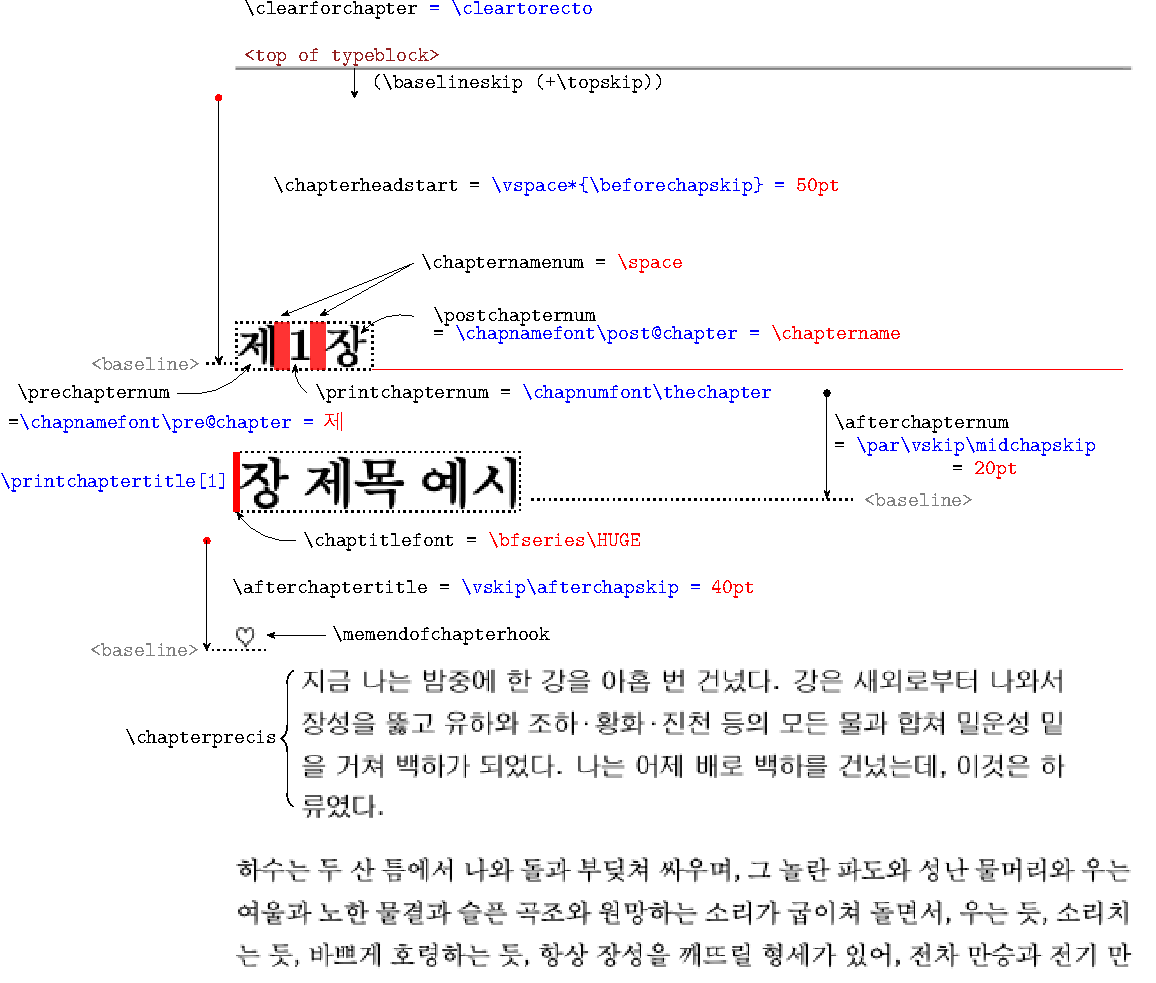
\includegraphics[width=\textwidth]{chapstyfig}
\caption{oblivoir의 장 표제 스타일}\label{fig:chapsty}
\end{figure}

\fref{fig:chapsty}\는 \textsf{oblivoir}의 장 표제 스타일에서 사용되는
매크로를 도시한 것이다.

KTUG 사설 저장소를 통하여 설치할 수 있는\footnote{%
	사설 저장소를 등록할 수 없는 상황이라면 직접 다운로드하라. 
	\url{http://ftp.ktug.org/KTUG/texlive/tlnet/archive/}
}
ob-chapstyles라는 패키지에는 몇 가지 memoir
chapter 스타일을 oblivoir화해둔 것이 있다. 이 자체를 그대로 써도 좋고 이를 자신만의 스타일을
만드는 데 참고하여도 좋을 것이다.

\subsection{한글 pagestyle}

oblivoir가 추가적으로 제공하는 페이지 스타일로 \texttt{hangul}이 있다.
\begin{boxedverbatim}
\pagestyle{hangul}
\end{boxedverbatim}

\subsection{crop mark: K style}

출판 현장에서 oblivoir를 이용하여 단행본을 제작하려 할 적에 \textsf{memoir}의
기본 crop mark가 너무 길어서 불평하는 경우가 있었다. 우리나라의 출판 현장에
알맞도록 조금 짧은 crop mark를 다음 명령으로 그릴 수 있게 하였다.
\begin{boxedverbatim}
\trimKmark
\end{boxedverbatim}

\subsection{\cs{ReleaseMacros} 명령}

여러 \LaTeX\ 패키지를 로드하여 쓰다 보면 어떤 명령이 이미 정의되었다는 에러를
만날 때가 있다. 이럴 때는 해당 패키지를 로딩하기 전에
\begin{boxedverbatim}
\ReleaseMacros{\XeTeX,\XeLaTeX}
\end{boxedverbatim}
과 같이 선언하여 이미 정의된 매크로를 무력화하는 시도를 해볼 수 있다.
둘 이상의 명령을 쉼표로 구분하여 지정할 수 있다.
이 명령은 preamble에서만 쓰게 되어 있다.


\subsection{oblivoirlist}

나열 환경의 아이템 간 간격을 제어하기 위하여 \verb|\oblivoirlist|와 
\verb|\oblivoirlists| 명령을 마련하였다. \verb|\oblivoirlists|는
해당 선언 이후 모든 나열환경을 \verb|\oblivoirlist| 간격으로 만든다.

\begin{itemize}\oblivoirlist
\item 배
\item 사과
\item 복숭아
\end{itemize}

다음 보기와 비교하여 보아라.

\begin{itemize}
\item 배
\item 사과
\item 복숭아
\end{itemize}

\footnotesinmargin
\textsf{memoir}의 \verb|\firmlist|와 \verb|\tightlist|는 여전히 동작한다.
\stepcounter{footnote}
\footnotetext{이 각주는 마진에 놓인다.} 
\addtocounter{footnote}{-1}

\subsection{sidefootnote와 footnotesinmargin}

oblivoir 2.0까지 \verb|\footnotesinmargin|이 동작하지 않던 문제를 고쳤다.\footnotemark

\verb|\sidefootnote|에서 발생하던 문제점도 해결하였다.\sidefootnote{이 각주는 사이드 풋노트이다.}

\footnotesatfoot
\textsf{memoir} 설명서에 설명된 것과 동일하게 동작한다.\footnote{상세한 것은 memoir manual을 볼 것.}

\subsection{[figtabcapt] 그림과 표의 캡션}

클래스 옵션으로 \texttt{[figtabcapt]}를 지시하면 기본적으로 다음과 같은 모양으로 캡션이 바뀐다.

\begin{boxedverbatim}
\caption{그림과 표의 캡션}
\end{boxedverbatim}
\begin{minipage}{\linewidth}
\centering
<그림 1> \quad 그림과 표의 캡션
\end{minipage}

\medskip

``그림 1'' 부분을 둘러싸는 delimiter를 다음 명령으로 바꿀 수 있다. 이 가운데
\verb|\obCaptionFont|는 캡션 텍스트에 영향을 미치는 명령이 아니고 라벨의 delimiter를
식자하는 데만 사용되는 폰트 명령이다.
\begin{boxedverbatim}
\renewcommand*\obCaptionnameOpen{[}
\renewcommand*\obCaptionnameClose{]}
\obCaptionFont{\sffamily\bfseries}
\end{boxedverbatim}
\renewcommand*\obCaptionnameOpen{[}
\renewcommand*\obCaptionnameClose{]}
\obCaptionFont{\sffamily}

\begin{figure}[h]
\caption{그림과 표의 캡션}
\end{figure}

이를 제외한 다른 부분, 이를테면 label과 caption text의 폰트를 바꾸는 것 등은 memoir의
해당 명령을 이용한다. 즉, \verb|\captionnamefont|, \verb|\captiontitlefont| 등을 이용하라는 것이다.

\section{보조 패키지}

\subsection{chaptertoc}

\marginpar{v3.0}
chaptertoc란 장 표제면에 그 chapter에 해당하는 절(section) 이하의 목록을
만드는 것을 말한다. 이 목적을 위한 별도의 패키지가 있고 oblivoir에서 해당 패키지를
활용하는 것도 가능하다. 한편 oblivoir v3.0은 \textsf{obchaptertoc}라는 부수
패키지를 제공하는데 이것은 \textsf{memoir}의 기능만을 이용하고 다른 패키지에
의존하지 않으면서 chaptertoc를 제작하게 한 것이다.
이 기능은 오직 \verb|\chapter|보다 높은 수준의 문서구분명령에서만 동작하며
\verb|\section| 이하 수준의 명령에 대해서는 고려하지 않았다. 따라서 \verb|[chapter]| 옵션이
주어진 경우에 유효하다고 하겠다.

\begin{boxedverbatim}
\usepackage{obchaptertoc}
%%
\chaptertoc
\end{boxedverbatim}

이 패키지는 원래 독자적으로 개발되었던 것으로 안내 문서를 따로 가지고 있다(한국어).
문서를 읽으려면
\begin{verbatim}
# texdoc obchaptertoc
\end{verbatim}

\subsection{mathleading}

oblivoir는 한국어 문서에 대하여 기본 행간을 넓혀서 조판하기 때문에 여러 줄 수식의 경우에도
그 영향을 받아서 행간격이 늘어지는 경우가 있었다.
\textsf{amsmath}의 여러 줄 수식에 대하여 이 문제를 조절할 수 있게 하는 \textsf{ob-mathleading}
패키지를 포함하였다. 따로 문서가 마련되어 있으므로 이를 참조하라.

\begin{boxedverbatim}
\usepackage{ob-mathleading}
\end{boxedverbatim}

문서를 읽으려면,
\begin{verbatim}
# texdoc ob-mathleading
\end{verbatim}

\subsection{oblivoir-misc}

\marginpar{v3.1}
시험적인 기능이나 그다지 중요하지 않은 명령을 포함하고 있는 
부수 패키지이다. 현재 다음 두 가지 명령이 정의되어 있다.

\begin{description}
\item[tikz pagenode] \texttt{tikz}를 로드했을 때 \texttt{current page}
노드가 memoir의 레이아웃과 미묘하게 엇갈리는 것을 보정해준다. 이것은 oblivoir-misc를 로드하면 (tikz가 불렸을 때) 자동으로 처리한다.
\item[\cs{texthl}] 한글 문자에 \texthl{하이라이트}해준다. 실험적인 기능으로
현재 \XeLaTeX 일 때에 정상 동작한다. 하이라이트할 색상은 \cs{obhlcolor}, 높이와
위치는 \cs{obhlheight}, \cs{obhlraisedim}을 재정의하여 설정할 수 있다.
\end{description}


\section{HTML 제작}

\textsf{lwarp}를 이용하여 HTML을 제작하려면 문서에 \textsf{lwarp} 
옵션을 주고 작성한다. 그 후,
\begin{verbatim}
lwarpmk html <file>.tex
\end{verbatim}
명령을 실행한다. MathJax 수식을 위해서는 
\begin{verbatim}
\documentclass[lwarp,lwarpoption={mathjax}]{oblivoir}
\end{verbatim}
와 같이 옵션을 줄 수 있다.

모든 문서가 원하는 모양대로 HTML로 만들어지지 않을 것이다. 특히
사용자화하여 복잡한 환경이나 명령을 만들어 쓴 경우에는 의도하지 않은
결과가 나올 수도 있음에 주의하라. 이 클래스의 \verb|lwarp| 옵션은
단지 \verb|lwarpmk| 명령을 부르기 위한 준비를 도와주는 것뿐이다.

\section{샘플 문서}

이 작은 안내서에 더하여 간단한 \obclass\ 샘플 문서를 하나 제공한다.
이 문서에서 여러 가지 memoir와 \obclass 의 기능을 살펴볼 수 있을 것이다.
oblivoir-test.tex을 컴파일해보고 소스를 검토해보시기 바란다.

%\subsection{fontspec 옵션과 수학 글꼴}\myLabel{sec:fontspec}{sec:폰트스펙}
%
%fontspec 패키지와 이를 확장한 mathspec 패키지를 이용하여
%수학 글꼴 일부를 바꾸고자 하거나 mathpazo와 같은 수학 글꼴 세트를
%적용하고자 할 경우가 있다. 이 때는 다음 두 가지 조치를 해야 한다.
%
%\begin{enumerate}[(1)]
%\item 클래스 옵션으로 [manualfontspec]을 선언한다.\footnote{%
%	2011/09/15 이전 버전에서는 [fontspec]이라는 이름이었다.}
%이 선언으로
%사용자는 fontspec을 자신의 책임 하에 로드할 수 있다. 심지어
%xltxtra나 mathspec과 같이 fontspec을 부르는 패키지를 별도로
%로드할 수 있다.
%\item 윗항의 fontspec 패키지 로드 후에 xetexko-xobfont 패키지를
%부른다. 이 설정 이후에야 \textbackslash setkormainfont 와 같은
%명령을 쓸 수 있게 될 것이다.
%\end{enumerate}
%이것은 mathfont를 조절하려면 fontspec의 옵션을 별도로 정의하여
%상세한 설정을 해야 할 경우가 있기 때문이다. 예컨대 mathpazo를 
%수학 기본 글꼴로 쓰려 한다면 다음과 같이 하는 것이 가능하다.
%\begin{boxedverbatim}
%\documentclass[manualfontspec]{xoblivoir}
%\usepackage{mathpazo}
%\usepackage[math,quiet]{fontspec}
%\usepackage[math,quiet,MnSymbol]{mathspec}
%\setmathsfont{Asana-Math}
%\setmainfont[Ligatures=Common]{Palatino Linotype}
%\usepackage{xetexko-xobfont}
%\end{boxedverbatim}
%이 예보다 간단하게 할 수 있는 것도 많다. 이 예는 설명을 위하여
%보인 것일 따름이다.
%위의 mathspec 대신 fontspec 패키지 문서에 나와 있듯이 \textbackslash setmathrm
%등의 명령으로 수학 폰트를 조절할 수 있다.
%
%2011/09/15 버전에서 이와 관련한 몇 가지 사항이 추가되었다.
%\begin{enumerate}[(a)]
%\item {[manualfontspec]} 옵션을 주었을 때는 위와 같은 방법으로 fontspec
%패키지를 수동 로드할 수 있다.
%\item {[fontspec=\{no-math\}]}와 같이 fontspec 패키지에 옵션을 미리 설정해줄
%수 있다. no-math 옵션을 주면 fontspec 명령들이 수식에는 영향을 끼치지 않으므로
%익숙한 CM-math 글꼴로 수식이 식자된다.
%\item {[preload=mathspec,preloadoption=\{math\}]}와 같이 preload할 패키지에
%넘겨줄 옵션을 preloadoption으로 지정할 수 있다.
%\end{enumerate}

%\subsection{옛한글과 세로쓰기}\myLabel{sec:oldhangul}{sec:올드한글}
% 옛한글 글꼴을 사용하려면 [oldhangul] 옵션을 주고 글꼴을 지정해야 한다.
% 세로쓰기는 사용가능하나, 아직 xoblivoir에서 조작하도록 하지는 않았다.
% \xetexko{} 매뉴얼에 옛한글 쓰기에 관한 간략한 소개가 있다.
%2010년 2월, \xetexko 의 옛한글 조판은 거의 완전한 수준에 이르렀다. 
%입력을 표준에 맞는 소위 `첫가끝' 코드로 하면서도 사용자 영역(PUA)에 옛한글이
%들어 있는 글꼴의 옛한글로 mapping이 가능해졌으며, GSUB 옛한글 글꼴(현재
%알려진 것으로는 은 바탕과 Microsoft Office 2002 Plus Pack의 옛한글 글꼴밖에 없다)을
%그대로 이용하여 옛한글 식자가 가능하다.
%
%이 역시 \xetexko 의 기능으로서 \xobclass는 더이상 할 일이 없어 이 절의 내용을 삭제한다.

%\subsection{amssymb}\myLabel{sec:ams}{sec:에이엠에스}
%amssymb 패키지를 로드하려 시도하면 몇 가지 명령이 이미 정의되어
%있다는 메시지가 나온다. 이 메시지를 줄이려면 amssymb 대신
%xob-amssymb를 usepackage하도록 한다.
%
%한편, LyX에는 amsmath와 amssymb 패키지를 자동으로 로드하는 기능이 있다.
%이 때문에 사용자가 xob-amssymb를 로드하려 해도 그보다 이전에 amssymb가
%LyX에 의해 로드되어 의도하는 결과를 얻지 못하는 경우가 있다. 이 때를 위하여
%[amsmath] 옵션을 마련해두었다. 이 옵션이 활성화되면 amsmath와 xob-amssymb를
%xoblivoir가 로드해준다. 
%
%\subsection{flowfram}\myLabel{sec:flowfram}{sec:플로프렘}
%fapapersize 및 flowfram 패키지와 함께 쓸 때, 첫 페이지의 pdf 사이즈만이 
%fapapersize로 지정한 것을 따라가지 않는 문제점이 있다.\footnote{%
%  이주호 님이 알려주셨음.}
%
%\xobclass 는 memoir의 페이지 출력 루틴을 조금 수정하여 대부분의 경우
%pdf 사이즈 충돌 문제가 해결되도록 해두었다.
%그러나 어떤 경우 pdf 파일의 첫 페이지와 이후 페이지의 사이즈가 불일치하는
%문제가 여전히 발생할 가능성이 있어 다음 옵션을 없애지 않았다.
%  
%[a4paper] 등 미리 정의된 페이지의 경우는 아무런 문제가 생기지 않는다.
%그러나 memoir 옵션으로 지정할 수 없는 사이즈,
%예컨대 190mm$\times$260mm pdf를 만들고 싶을 때는 어떻게 하는가?
%\xobclass 에게 페이지 사이즈를 강제로 알려주는 방법이 있다.
%\begin{boxedverbatim}
%\documentclass[<other options>,fawd=190mm,faht=260mm]{xoblivoir}
%\usepackage{fapapersize}
%\usefapapersize{190mm,260mm,30mm,*,40mm,*}
%\usepackage{flowfram}
%\end{boxedverbatim}
%이제 첫 페이지의 사이즈도 두번째 이후의 것과 같아졌을 것이다.
%
%\subsection{preload}\myLabel{sec:preload}{sec:프리로드}
%일부 패키지 중에는 이따금 memoir 클래스 자체보다 미리 로드되어야 하는 것이 있다.
%대표적인 예가 아랍어를 식자할 때 빼놓을 수 없는 bidi 패키지이다.
%이와 같이 memoir보다 먼저 로드해야 하는 패키지를 쓸 때 다음과 같이 한다.
%\begin{boxedverbatim}
%\documentclass[preload={bidi}]{xoblivoir}
%\end{boxedverbatim}
%
%preload할 패키지에 전해줄 옵션은 다음과 같이 설정한다.
%\begin{boxedverbatim}
%\documentclass[preload={mathspec},preloadoption={math}]{xoblivoir}
%\end{boxedverbatim}
%
%moreverb의 경우도 이렇게 하면 되므로 이제 의미가 없어진 옵션이 되었지만 종래
%작성된 문서와의 호환을 위해서 없애지는 않았다.
%
%\subsection{moreverb}\myLabel{sec:moreverb}{sec:모아버브}
%이 옵션은 pstricks를 사용하기 위하여 pdfm\-tricks를 이용하려 할 때
%필요하다. pdfm\-tricks는 moreverb, graphicx, (x)color 패키지가 미리
%로드되어야 동작하는데, 이 중 graphicx와 xcolor는 문제가 없지만
%oblivoir(memoir)에서 moreverb는 \textbackslash usepackage 로
%로드하면 memoir의 일부 명령과 충돌한다.
%이 충돌을 해결해주는 옵션이며, 이 옵션을 준 후에 moreverb를 별도로
%로드할 필요 없다. moreverb는 \myPageREF{sec:preload}{sec:프리로드}에서 설명하는
%preload로 미리 로드하는 방법이 있으므로 사실상 obsolete인 옵션이다.
%
%\subsection{microtype}\myLabel{sec:microtype}{sec:마이크로타입}
%현재까지 \XeTeX 은 pdf\TeX과 Lua\TeX 의 microtype 기능을 엔진 수준에서 지원하지 않는다.
%그러나 \xetexko 는 xetexko-hanging이라는 기법을 이용하여 온점과 반점을 판면 밖으로 밀어냄으로써
%margin kerning과 비슷한 효과를 줄 수 있게 하는 재미있는 기능을 제공한다.
%이 옵션은 이름은 microtype이지만 실은 xetexko-hanging을 활성화하는 역할을 한다.
%이 문서가 이 기능을 활성화하여 작성되었다.
%
%\subsection{hyperref, xcolor}\label{sec:hyperrefxcolor}
%LyX 을 쓴다거나 할 때 \XeTeX 을 위해서 hyperref의 [unicode] 옵션을 
%꺼주어야 할 때가 있다. 이를 위해서 hyperref 패키지에 미리 넘길 옵션을 지정할 수 있게 
%하였다.
%\begin{boxedverbatim}
%\documentclass[hyperref={unicode=false}]{xoblivoir}
%\end{boxedverbatim}
%
%필요에 의해 xcolor 패키지에 대해서도 비슷하게 할 수 있도록 해두었다.

\section{첨언}
\xobclass{} 사용이 어느 정도로 쉬운가 하면, 나는 맨처음 이 문서를
LyX에서 작성하여 export한 다음, 두 줄 정도를 지우고 폰트
설정명령만을 써넣었다. 그래도 훌륭한 \XeLaTeX\ 문서가 만들어졌던
것이다.

이 글을 쓰기 시작할 때만 해도 \xetexko{}와 \xobclass{}는
완성되어 있지 않았다. 그러나 지금은 일반적인 문서를 작성함에 있어서
불편이 없을 정도가 되었다.

\bigskip

돌이켜보면, 한글을 \TeX\ 문서에 사용할 수 있다는 사실 자체가
신기했던 그 때로부터 20여년이 흘렀다. 본격적인 한글\LaTeX\ 시스템들이
나오기 시작했던 1990년대 중반으로부터 헤아려도 십수 년,
이 기간 동안 한글이라는 문자 체계를 식자하기 위해 지불해야 했던
엄청난 노력과 자원을 생각하면 금석지감이 없지 않다.

Lua\TeX 과 \XeTeX 이라는 유니코드 텍 엔진의 등장은, 이러한 모든
노력들을 일시에 해결해버렸다. 이제 한글 문자의 식자는 더이상
문제가 되지 않는다.
그러나 한글 문서다운 한글 문서, 한글 문서의 타이포그래피의 완성을
위한 길은 아직도 요원하다. 단순히 “글자를 찍는” 문제가 해결되었다고
해서 모든 일이 끝난 것은 아닌 것이다. 단지 더 생산적인 문제를
더 잘 구현할 수 있는 바탕이 갖추어진 것일 뿐이라고 생각한다.


\section{변경 이력}


2022년의 3.1 버전은 fapapersize에 새로운 명령을 추가하고 약간의
개선된 기능을 포함하였다. 

\noindent
2021년의 3.0 버전은 상당히 많은 버그와 의도와 다른 동작을 수정하고 새로운 
기능을 추가하였다.

\noindent
2020년의 2.2 버전은 그 동안 알려진 몇 가지 버그를 수정하고 약간의 기능을
추가하는 데 그쳤다.

% \section{알려진 문제점}

% 아래 문제점과 버그들은 다음 버전에서 해결하도록 노력할 것이다.

% \begin{enumerate}[(가)] \tightlist
% % \item ExternalLocation 옵션을 활성화하는 설정과 그렇지 않은 설정을 함께 쓸 때
% % ExternalLocation 명령이 순서상 먼저 나와야 한다. 

% \item 윈도우즈 폰트 네임과 다른 리눅스 및 매킨토시의 폰트 이름 호출이
% 실패하는 경우가 있다. 다행히 은 글꼴의 경우는 문제없으나, 은 글꼴은 반드시
% 최신 버전이어야 한다. 우분투 등의 리눅스에서 패키지로 설치해주는 기본 설치
% 글꼴은 때로 문제를 일으킨다. 이것은 저자가 어찌해볼 수 있는 문제가 아니다.
% \end{enumerate}

% 한글 기호 문자 일부는 한자 영역에 배정하였다. 한자가 없는 한글 글꼴을
% 본문 기본 서체로 지정하는 경우를 위한 것이다. 그러나 이 문제는 아직
% 확정된 것이 아니며 좀더 테스트를 거쳐서 결정할 일로 보인다.

%%\section{이 문서의 폰트 사용 설정}
%%
%%이 문서의 폰트 사용 설정은 다음과 같다.
%%\begin{boxedverbatim}
%%\setmainfont[Mapping=tex-text]{Bradley Hand ITC}
%%\setmonofont[Scale=.85]{Consolas}
%%\setkormainfont(문화 궁서 Std L){문화 궁서 흐림 Std L}(){네이버사전}
%%\setkormonofont{은 필기}
%%\setmonoscale{0.9}
%%\end{boxedverbatim}

%%%\section{버전 인포}\myLabel{sec:versioninfo}{sec:버전인포}
%%%
%%%\begin{enumerate}\tightlist
%%%\item 이 초간단 매뉴얼은 xoblivoir 2011/09/15 버전에 일치한다.
%%%\item 이 초간단 매뉴얼은 xoblivoir 2010/02/10 버전에 일치한다.
%%%\item 이 초간단 매뉴얼은 xoblivoir 2008/12/03 버전에 일치한다.
%%%\item 이 초간단 매뉴얼은 xoblivoir 2008/11/24 버전에 일치한다.
%%%\item 이 초간단 매뉴얼은 xoblivoir 2008/11/09 버전에 일치한다.
%%%\item 이 초간단 매뉴얼은 xoblivoir 2008/10/23 버전에 일치한다.
%%%\item 이 초간단 매뉴얼은 xoblivoir 2008/10/22 버전에 일치한다.
%%%\item 이 초간단 매뉴얼은 xoblivoir 2008/10/12 버전에 일치한다.
%%%\item 이 초간단 매뉴얼은 xoblivoir 2008/10/11 버전에 일치한다.
%%%\end{enumerate}
%%%
%%%%%% 한자 테스트
%%%이 매뉴얼은 Notepad++로 編輯하였다. 다 좋은데 Notepad++의
%%%KCmenu plug\-in에 xelatex 實行 命令 短縮키가 없어서 不便했다.
%%%그러던 것이 최근 새로운 단축키가 생김으로써 훨씬 편하게 작업할
%%%수 있게 되었다.
%%%
%%%%이 글을 더 줄인 \bnm*{極超簡單 매뉴얼}을 究想中이다.

\end{document}
